%%%%%%%%%%%%%%%%%%%%%%% file template.tex %%%%%%%%%%%%%%%%%%%%%%%%%
%
% This is a general template file for the LaTeX package SVJour3
% for Springer journals.          Springer Heidelberg 2006/03/15
%
% Copy it to a new file with a new name and use it as the basis
% for your article. Delete % signs as needed.
%
% This template includes a few options for different layouts and
% content for various journals. Please consult a previous issue of
% your journal as needed.
%
%%%%%%%%%%%%%%%%%%%%%%%%%%%%%%%%%%%%%%%%%%%%%%%%%%%%%%%%%%%%%%%%%%%
%
% First comes an example EPS file -- just ignore it and
% proceed on the \documentclass line
% your LaTeX will extract the file if required
%\begin{filecontents*}{example.eps}
%%%!PS-Adobe-3.0 EPSF-3.0
%%%BoundingBox: 19 19 221 221
%%%CreationDate: Mon Sep 29 1997
%%%Creator: programmed by hand (JK)
%%%EndComments
%gsave
%newpath
%  20 20 moveto
%  20 220 lineto
%  220 220 lineto
%  220 20 lineto
%closepath
%2 setlinewidth
%gsave
%  .4 setgray \textit{fill}
%grestore
%stroke
%grestore
%\end{filecontents*}
%
%\documentclass{svjour3}                     % onecolumn (standard format)
%\documentclass[smallextended]{svjour3}     % onecolumn (second format)
%\documentclass{svjour3}        % twocolumn
\documentclass[smallcondensed]{svjour3} %requested in Journal 
\smartqed  % flush right qed marks, e.g. at end of proof
%


\usepackage{graphicx}
\usepackage{palatino,epsfig,latexsym}
\usepackage{amsmath,amsfonts,amssymb,color}
\usepackage{graphicx}
\usepackage{algorithm}
\usepackage{algorithmic}
\usepackage{subfigure}
\usepackage{multirow}
\usepackage{bbm}
\usepackage{url}
\usepackage{float}
\renewcommand{\textfraction}{.01}
\renewcommand{\bottomfraction}{.99}
\renewcommand{\topfraction}{.99}
%\setcitestyle{square}
\sloppy
%
\begin{document}

\title{The EvoSpace Model for Pool-Based Evolutionary Algorithms}
% a framework that does what? That is the best for what? Is this a
% publicity paper or something more? What are you going to say about
% this framework? Introducing? Assessing? - JJ


%\titlerunning{Short form of title}        % if too long for running head

\author{Mario Garc\'ia-Valdez         \and
        Leonardo Trujillo \and
		Juan-J Merelo\and
		Francisco Fern\'andez-de-Vega\and
		Gustavo Olague
		}

%\authorrunning{Short form of author list} % if too long for running head

\institute{Mario Garc\'ia-Valdez \at
           Instituto Tecnol\'ogico de Tijuana, Calzada Tecnol\'ogico S/N, Tijuana, BC, 22414  \\	
              \email{mario@tectijuana.edu.mx}           %  \\
%             \emph{Present address:} of F. Author  %  if needed
           \and
           Leonardo Trujillo \at
           Instituto Tecnol\'ogico de Tijuana, Calzada Tecnol\'ogico S/N, Tijuana, BC, 22414  \\
           \email{leonardo.trujillo@tectijuana.edu.mx} \\	
           Website: www.tree-lab.org \\ 
			\and
			Juan-J Merelo
	         \at
	        Departamento de Arquitectura y Tecnolog\'ia de Computadores University of Granada, Spain\\
	\email{jmerelo@geneura.ugr.es}
			\and
			Francisco Fern\'andez-de-Vega
			\at
			Grupo de Evoluci\'on Artificial, Universidad de Extremadura, Spain\\
	\email{fcofdez@unex.es}	
		\and
		Gustavo Olague
		\at
		Centro de Investigaci\'on Cient\'ifica y de Educaci\'on Superior de Ensenada\\
\email{olague@cicese.mx}		
}

%\date{Received: date / Accepted: date}
% The correct dates will be entered by the editor


\maketitle

\begin{abstract}
This work presents the EvoSpace model for the development of pool-based evolutionary algorithms (Pool-EA).
Conceptually, the EvoSpace model is built around a central repository or population store, incorporating some of the principles of the tuple-space model
and adding additional features to tackle some of the issues associated with Pool-EAs;
such as, work redundancy, starvation of the population pool, unreliability of connected clients or workers, and a large parameter space.
The model is intended as a platform to develop search algorithms that take an opportunistic approach to computing,
allowing the exploitation of freely available services over the Internet or volunteer computing resources within a local network.
A comprehensive analysis of the model at both the conceptual and implementation levels is provided,
evaluating performance based on efficiency, optima found and speedup, while providing a comparison with a standard EA and an island-based model.
The issues of lost connections and system parametrization are studied and validated experimentally with encouraging results,
that suggest how EvoSpace can be used to develop and implement different Pool-EAs for search and optimization.    

\keywords{Pool-based Evolutionary Algorithms \and Distributed Evolutionary Algorithms\and Heterogeneous Computing Platforms for Bioinspired Algorithms  \and Parameter Setting}

\end{abstract}

\section{Introduction}
\label{sec:intro}
%Over the last decade,  %I'd change that to concrete dates. Nobody
                       %knows $n$ years from now which decade was that
                       %- JJ
%the landscape in computing technology has undergone a noticeable shift, moving away from isolated,
%serial, single-tenant and synchronous systems, towards distributed,
%ubiquitous, multi-tenant and shared computing resources,
%exploiting network infrastructure and what is known as the Cloud Computing model\cite{cloud, varia2008cloud}.
%This shift is not easy to make, %for whom? which shift? - JJ
% several examples should be mentioned here, including one that refers
% to the exploitation of computing resources available on the Internet
% which is mentiones in Related work - JJ 
% it requires a dedicated and coordinated effort to migrate systems
% from one paradigm to another. % why do you have to migrate? You can
                               % use both. I'd rather focus on the
                               % need to adapt algorithms and
                               % implementation methodologies - JJ

In the early 1990s Foster and Kesselman defined the term Grid Computing \cite{Foster:1998}, referring to an infrastructure designed to enable resource sharing from multiple locations, while also being coordinated to reach a common goal. Early Grid applications were initially motivated by the particular demands of advanced science and engineering applications \cite{Baxevanidis:2002}, seeking a low cost alternative to dedicated data centers or clusters. What distinguished grid computing from conventional high performance computing systems, was that grids tend to be more loosely coupled, heterogeneous, and geographically dispersed \cite{Foster:1998}. With the ubiquity of the Internet, nowadays researchers have access to vast  computational resources which are disperse and available using various technologies, including cloud computing \cite{cloud,varia2008cloud}, peer-to-peer (P2P) networks  \cite{Oram:2001}, and web services \cite{Curbera:2002}.

On the other hand, Evolutionary Computation (EC) researchers require powerful computational resources, since EC algorithms tend to be computationally demanding. EC algorithms can benefit from grid computing infrastructures, by designing them as parallel, distributed and asynchronous systems. Several Evolutionary Algorithms (EAs) have been proposed that distribute the evolutionary process among heterogeneous devices, not only among controlled nodes within in-house clusters, but also in those outside the data center, in users' web browsers, smart phones or external cloud based virtual machines. This reach out approach allows researchers the use of low cost computational power that would not be available otherwise.
However, such systems present several noteworthy challenges, such as the need to manage heterogeneous and unreliable computing resources,
low bandwidth communications, as well as security and privacy issues. 
 
This paper is part of an ever-growing effort in the field of EC to develop algorithms following this opportunistic approach to computing, allowing the exploitation of freely available services over the Internet or volunteer computing resources. To enable this arbitrary plug-in and plug-out of computational resources for distributed EAs, a new pool-based architecture has been proposed \cite{sofea1,sofea2,sofea3,PoolvsIsland,Evospace,Musart,FreeLunch,Fire}.
The basic idea behind Pool-based EAs (Pool-EAs) is that all the participants of the distributed algorithm share a common population stored in a central server, from which each participant can pull a set of tasks or data from the server, perform some work and then return the results back to the server. Pool-EAs differ from the closely related island model, mainly with regards to the responsibilities that are assigned to the server.
In the island model the server is usually responsible for the interaction and synchronization of all the populations,
while in a Pool-EA the server only receives stateless requests from isolated participants or clients. 
In this way, Pool-EAs are capable of an ad-hoc collaboration of computing resources.
However, there are still several open issues that need to be addressed for the deployment of a Pool-EA system, particularly:
\begin{enumerate}
	\item Work Redundancy: in a Pool-EA, two or more participants often take the same tasks or data to work on, possibly duplicating
	computational effort.
	\item Starvation of the Population Pool: this happens when there are no more tasks or data in the server, participants must wait idly for tasks to become available.
	  
	%\item Participants are unaccountable and essentially anonymous: participants occasionally malfunction and return incorrect results. 
	
	\item Participants are Unreliable: participants might abandon their work, they might malfunction or loose their connection, thus delaying or failing to return their results to the server.
	\item Parametrization: The number of parameters is incremented with respect to a traditional EA, with specialized parameters such as the number of tasks pulled by each participant, the size of the pool, the amount of time the server waits for a result, among others. Moreover, participants could also have internal parameters, that could be set homogeneously or heterogeneously.
	\item Single Point of Failure: conceptually, there is a single central server managing the pool, a single point of failure.  	
	%\item Asynchronous Behavior: Asynchronous systems could be hard to implement.
\end{enumerate}
        
Issue (5) is a deployment problem, that can be addressed at the technological level, without regards to the evolutionary model.
Most of the other issues have been extensively studied in distributed systems research.
For instance, Gelertner and Carriero \cite{linda} developed a model that addresses issue (1), introducing the concept of a tuple space, a repository of tuples or shared objects, that can be accessed concurrently by several processes. This tuple space functions as a communication and coordination mechanism between distributed processes that interact with each other through these shared tuples. A distinctive characteristic of this model is that in order to change the state of a tuple, a process needs to atomically remove the tuple from the space and place it back only after it has released it; this inherently provides mutual exclusion since another process cannot access a tuple while it is being used. A benefit of such a model for Pool-EAs is that it forbids two clients from duplicating work. 

This papers presents the EvoSpace Model (ESM), a conceptual framework for the development of Pool-based EAs \cite{Evospace}.
The ESM is built around a central repository or population store, incorporating some of the main principles of the tuple-space model.
However, the ESM is not simply an implementation of the tuple-space model for EAs,
since it incorporates additional mechanisms and concepts specifically tailored to address each of the above listed issues for Pool-EAs.
In particular, issue (1) is solved by defining the interaction between distributed workers and the centralized pool using the tuple space principles.
Issue (2) is solved by incorporating a reinsertion process, that determines when the central Pool will be starved, and takes proper corrective measures.
Moreover, experimental work presented in this paper suggests that the ESM is not hampered by issues (3) and (4).


The ESM has two main components, a set of EvoWorkers and a single instance of an EvoStore. The EvoStore container manages a set of objects representing individuals in a EA population. EvoWorkers pull a subset of individuals from the EvoStore, making them unavailable to other workers. Moreover, individuals are removed from the EvoStore as a random subset or sample of the population, this differs from the tuple-space paradigm which removes only those tuples matching a pattern-based query. The ESM also includes a reinsert operation which allows a sample once removed from the population to be reinserted on-demand. Intuitively this can be seen as if individuals once removed from the EvoStore changed to a phantom state, and if needed they could be brought back to life. Once an EvoWorker has a sample to work on, it can perform a partial evolutionary process, and then return the newly evolved subpopulation to the EvoStore where the new individuals replace those found in the original sample; at this point replaced or reinserted individuals can be taken by other clients. Another possibility is that  EvoWorkers pull a sample just to change the state of individuals and then return the sample, all of this without executing an EA loop. Example of this scenario can be found in interactive evolutionary algorithms, where users pull a sample of individuals from the EvoStore container to assign a fitness value \cite{Musart,Fire}.  
EvoWorkers perform their tasks in an asynchronous manner, contrasting with the traditional sequential and synchronous evolutionary model followed by most EAs. Indeed, new evolutionary models, such as the ESM, allow the design of Pool-EAs that include algorithmic features present in natural evolutionary systems, but that are difficult to reproduce in sequential and synchronous processes \cite{eiben}.

This paper presents a detailed description of the ESM, building upon our previous contributions \cite{Evospace,FreeLunch},
and providing a comprehensive analysis of the system at both the
conceptual and implementation levels.
Furthermore, several design issues are addressed, that illustrate the robustness of the ESM.
Particularly, the problems of lost connections and system parametrization are studied and validated experimentally, with
encouraging results, that suggest how EvoSpace can be used to develop and implement different Pool-EAs for search and optimization.

%Firstly, distributed systems have to account for unreliable clients, and how lost connections can compromise system performance,
%an issue that is experimentally evaluated in this paper.
%
%Secondly, by performing the evolutionary process over a number of distributed workers, the system's parameter space grows exponentially,
%thus greatly enhancing the undesirable feature of most EAs, that of tuning and parameterizing the algorithm for a new problem.
%
%This issue is addressed by using a simple, but efficient,
%parametrization method originally developed for Island model EAs
%\cite{fuku2}.
% A small panorama of Pool-EAs should be introduce here, showing the
% different options and how pool-based models fit within them - - JJ

The remainder of the paper proceeds as follows.
First, a comprehensive discussion pertaining to related work is presented in Section \ref{sec:related}.
Afterwards, the ESM is detailed in Section \ref{sec:evospace} and a reference implementation is presented in Section \ref{sec:ref}.
Three experimental validations are performed in Section \ref{sec:exp1} using genetic algorithm benchmarks:
first, the ESM is compared with another distributed EA to illustrate some of its
strengths and weaknesses; second, the ESM is tested with regards to diversity and scalability;
and finally, a cloud based deployment is used to evaluate the system's performance and communication costs.
Section \ref{sec:overcome} deals with two general issues associated with Pool-EAs in general, and ESM in particular,
and proposes useful solutions which are validated experimentally.
Finally, a summary of this work, conclusions and future work are presented in Section \ref{sec:conclusions}.
 

\section{Related Work}
\label{sec:related}
In terms of parallelizing EAs, a large body of work has developed a variety of parallel models, with
important practical and theoretical results \cite{parallelEA}.
However, our work focuses on the goal of distributing an EA over a grid, a much less explored topic in EA research.
In particular, this section will contextualize Pool-EAs within the more general research area of distributed EAs,
to correctly frame the contributions made in the proposed model.

Probably the most unobtrusive way to distribute an EA over an heterogeneous collection of computing resources is to run an EA over the Internet using web browsers.
For instance, Klein and Spector \cite{spector:2007} and Merelo et al. \cite{merelo:2008} developed EAs that distribute fitness function evaluations over the web using Javascript on the client machine, such an approach comes with the benefit that connected clients do not need to install any special software on their systems,
since the code is directly executed on the browser.
Another recent example is given by Cotillon et al. \cite{cotillon:2012}; they take the idea of browser-based EAs to the Android OS, which can be
executed on a large number of mobile devices.
Other common examples of web-based EAs come from the area of interactive evolution, where users visit a web page, browse candidate individuals
and participate in the evolutionary process by evaluating individuals in artistic design problems \cite{Musart,Fire,langdon:2004,picbreeder}.
However, in these works the EA process is not necessarily executed on the browsers themselves, they are mostly used as practical interfaces
to obtain user input, while the actual search is performed on the server.


Other researchers have exploited other network-based technologies to distribute an EA over a set of computing nodes.
For instance, Cole et al. \cite{MilkyWay} uses the popular Berkeley Open Infrastructure for Network Computing (BOINC) to distribute an EA,
using the volunteer computing model, where connected clients share idle CPU cycles with a research project.
Another example is the work of Fern\'andez-de-Vega et al. \cite{nc}, who also distributes multiple EA runs using a volunteer computing network through BOINC.
Garcia-Arenas et al. \cite{garcia2011} used the popular file sharing service Dropbox as a storage server for an EA.
Jim\'enez-Laredo et al. \cite{garcia2011} uses a P2P architecture to distribute a Genetic Programming (GP) algorithm over a network.
Similarly, the DREAM framework presented in \cite{DREAM} also distributes an EA using a P2P network based on mobile multi-agent systems.
Another example is the ParadisEO object-oriented framework for the reusable design of parallel and distributed metaheuristics, including EAs, developed
by Cahon et al. \cite{ParadisEO} using a distributed model based on the Farmer/Worker paradigm.
Recently, researchers have also begun to fully integrate EAs into the Cloud computing model.
For instance, the Eureqa \footnote{http://www.nutonian.com/} GP-based modeling tool, originally developed by Schmidt and Lipson \cite{free-form},
and now marketed by Nutonian, easily integrates with Amazon's EC2 Cloud service for faster computation.
A better integration of EAs with Cloud models has already been pursued by some researchers.
Two noteworthy examples are the Offspring framework by Vecchiola et al. \cite{VecchiolaCORR}
and the FlexGP system developed by Sherry et al. \cite{FlexGP}.
Offspring runs a multiobjective EA that is executed on Aneka Enterprise Clouds using a simple distribution logic that makes the use of the cloud
transparent for the user, developed on top of the task model with a plug-in architecture.
FlexGP is probably the first large scale GP system that runs on the cloud, using an Island model approach and implemented over
Amazon EC2 with a socket-based client-server architecture.
Other recent contributions include several tools and libraries designed to distribute an EA over the Cloud using a global queue of tasks and a Map-Reduce
implementation \cite{FlexGP}.


All of these works show great promise in extending EAs towards modern computing models.
However, they focus on exploiting current distributed computing technologies to enhance EA performance, while maintaining the same basic evolutionary model.
In other words, in terms of the search the EA might perform the exact same process, even if it is done more efficiently through distributed computing technologies.
On the other hand, the current work deals with a novel EA model introduced by Pool-EAs.
What is particularly interesting in a Pool-EA, is that they are explicitly designed to exploit a distributed computing framework, while also employing
an EA model that incorporates non-traditional search dynamics.
In a Pool-EA, the evolving population is stored in a centralized repository or store, while distributed clients asynchronously extract a subset
of individuals and return a new subset of individuals after performing the actual search operators.
Pool-EAs are related to more general systems, such as the A-Teams system proposed in \cite{ateam}, a problem-solving multi-agent architecture based on a strongly cyclic network.
G. Roy et al. \cite{roy:2009} also developed a multi-threaded system with a shared memory architecture
that is executed within a distributed environment, where the evolving population of a GA is stored in a centralized pool or database.
Another example is developed by Bollini and Piastra \cite{bollini:1999}, who proposed a system that decouples population storage from the actual evolutionary operations.

Pool-EAs are closely related with Island-Model EAs (IMEA) \cite{cantu} with several noteworthy differences \cite{PoolvsIsland}.
In an IMEA, each island represents a partially independent evolutionary process, with a periodic exchange of
individuals following a synchronized and coordinated protocol, using a fixed topological structure.
On the other hand, a Pool-EA does not employ such a coordinated interaction scheme, workers perform an evolutionary process
using a sample of individuals taken from the central pool.
Moreover, the manner in which workers interact with the central pool is completely random and asynchronous.
These conceptual difference illustrate how a Pool-EA offers a much simpler approach towards the development of a distributed evolutionary
search, eliminating some of the parameters or design choices that are not easy to determine in an IMEA application
(such as the number of islands, migration strategies and communication topologies).
In other words, a Pool-EA allows for the deployment of an ad-hoc distributed EA, where connected clients can connect and disconnect from the
EA process without strict prior restrictions or system configuration.
However, whether or not these differences provide any performance advantages can be seen as an empirical question, one that is considered
in the experimental sections of this paper.

The most complete Pool-EA model proposed thus far is the SofEA algorithm by Merelo et al. \cite{sofea1,sofea2,sofea3}.
SofEA is an evolutionary algorithm mapped to a central CouchDB object store. It provides an asynchronous and distributed search process,
where the four main evolutionary operators are completely decoupled from the evolving population; these are: Initialization, Evaluation, Reproduction and Elimination.
The last three processes can be executed in any order and in any given time step, and more than a single Evaluator and Reproducer can be
executed concurrently.
EvoSpace shares several similarities with SofEA, but it also has several noteworthy differences.
First, while SofEA also presents a distributed and asynchronous model, the evolutionary process is still carried out on the central repository.
On the other hand, in EvoSpace evolution is carried out locally on each client, as if small sub-populations are periodically isolated, evolved and then returned to the central store.
Second, while both systems attempt to decouple population storage from the search operations, SofEA maintains a fine-grained control of each individual
within the population that limits the ability of each to interact with remote clients.
For instance, once an individual is evaluated in SofEA, its fitness cannot be reassigned based on a future evaluation,
this limitation is particularly important in the development of interactive systems where several users could provide input regarding the quality of a solution \cite{Musart}.
Thirdly, since SofEA considers each individual as unique, it does not allow duplicates to appear within the evolving population, something that is useful for diversity preservation but that might curtail the exploitation capability of the EA, since multiple copies of a particularly high-quality solution cannot be present.
Furthermore, if an individual dies (or is eliminated), then another copy of it cannot be reintroduced into the population,
even if it might be useful at a later stage of the search.
Finally, by using the individual chromosome as ID, it appears problematic to extend SofEAs to more complex representations such as GP,
an extension that is easily accomplished with EvoSpace.

\section{The EvoSpace Model} %System or framework? Is EvoSpace a
                              %framework implementing a model or
                              %system? You should be more precise
                              %about this - JJ
\label{sec:evospace}
The ESM is a conceptual framework for the development of Pool-based EAs. Figure \ref{fig:evo} shows a graphical illustration of the main components and data-flow within the ESM. The main components are: the EvoStore population container, remote clients called EvoWorkers, and the stored objects or Individuals of an EA search.
Each of these components are defined in the following subsections.

%Basically, EvoSpace consists of two main components. % You can't keep
                                % re-defining EvoSpace. Later on you
                                % say it's based on the tuple space
                                % model. And the graph above includes
                                % only one EvoSpace box: population
                                % store. 

\begin{figure*}[t]
    \centering
        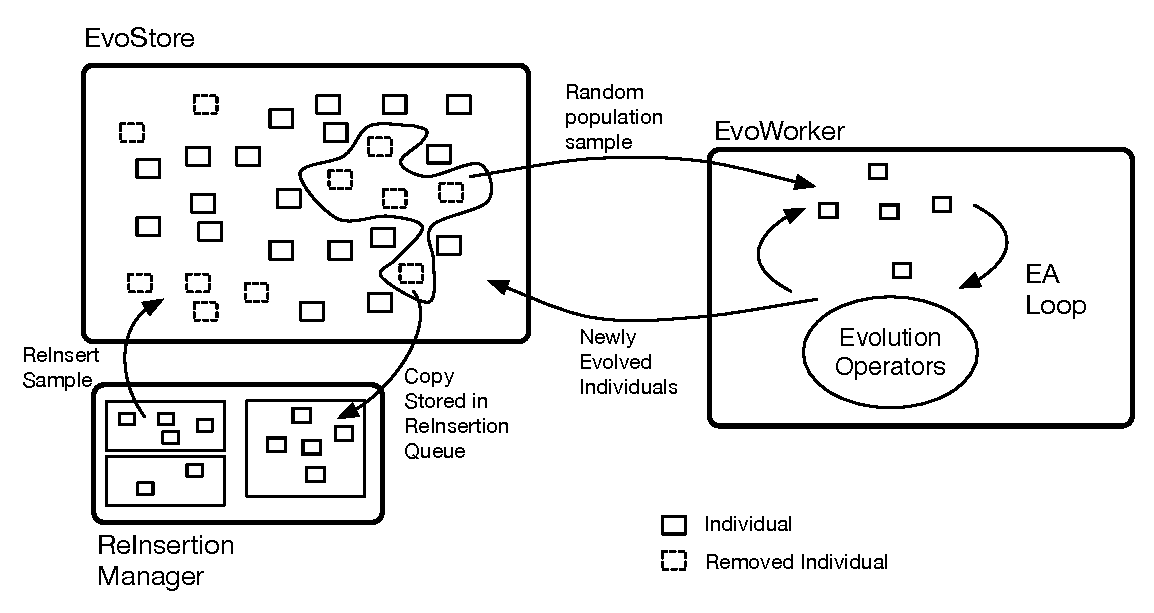
\includegraphics[width=12cm]{evospaceExample.eps}
    \caption{Main components and dataflow within the EvoSpace model.}
    \label{fig:evo}
\end{figure*}

% In all these sections there's a lot of description but very little
% fo the rationale behind them. Why did you do it this way? That
% applies to sections above and below - JJ
\subsection{The EvoStore container}
\label{sss:container}
%This should be included in the Fig 1. Is it the same as the
%Population Store? In Fig. 2 EvoSpace is only the population store. 
The EvoStore is an associatively addressed memory space shared by several processes following the principles of the tuple-space model, which can be described as a distributed shared memory (DSM) abstraction, organized as a bag of tuples.
A tuple $t$ is the basic tuple space element, composed by one or more fields and corresponding values. In this model, the basic operations that a process can perform is to insert or withdraw tuples from the tuple space. % You could say here
                                % that's it's different from SofEA,
                                % since SofEA is an _array_ of tuples
                                % that can't be accessed randomly - JJ 
An EvoStore provides a set of interface methods that operate over a set of objects $ES$, which can be seen as an independent EA population. If multiple populations are needed, each one must have an index as in $ES_i$. For simplicity in this description, we assume an EvoStore has a single population $ES$. Objects in $ES$ represent individuals in the population (these are defined in the next subsection), they can be removed and replaced from $ES$ using a specified set of methods. However, the ESM is different from other tuple space implementations in the sense that retrieving and reading objects from $ES$ are defined as random operations. Retrieving a single objects is not of high interest when accessing the EvoStore, instead samples of the population are desired, a key difference with the SofEA approach \cite{sofea1,sofea2,sofea3}.
The methods provided by the EvoStore container are the following:

\begin{itemize}
 \item \textbf{Read(n):} This method returns a random set $A$ of objects from $ES$, with $|A|=n$ and $A\subset ES$, if $n< |ES|$, the method returns $ES$ otherwise. When using this method, objects are not removed from $ES$ meaning that they are intended for read-only operations.
This method is useful to analyze the evolving population without interfering with the search, to compute performance measures online.

\item \textbf{Take(n):} Returns a random set $A$, following the same logic used for $Read(n)$. However, in this case the set $A$ is removed from $ES$, the contents of the EvoStore are then given by $ES = ES \setminus A$.
We define  $A_i$ as the set returned by the $i-th$ $Take()$ operation.
The objects taken are also copied to a new set $S_i$ of removed samples and stored
within a temporary collection $\mathcal{S}$ on the server, implemented as a priority queue. Sets $S_i \in \mathcal{S}$ can then be reinserted to $ES$ if necessary.  
 
 \item \textbf{ReInsert(i):} This method is used to reinsert the subset of elements removed by the $i-th$ $Take()$ operation,
  such that the contents of EvoSpace are now $ES \cup S_i$ if $S_i \in \mathcal{S}$, $ES$ is left unchanged otherwise.
  In other words, the method ReInserts previously taken samples from the population store.
  The ReInsert method can be triggered when a worker loses its connection to the server or when the population size gets below a threshold, this prevents the starvation
  of the population pool and also compensates for lost work. Other distributed algorithms normally use a random insertion technique, but this might negatively impact the search process if good solutions are lost.
      
 \item \textbf{Insert(A):} This method represents the union operation $ES \cup A$, where $A$ is a set of individuals.
 This method is normally used to initialize the population, with a randomly generated set of individuals.
 This differs from ReInsert, which introduces previously taken individuals.
 Section \ref{sec:overcome}, analyzes the effects of using Insert (with a random set of individuals) instead of ReInsert (with individuals from a previously
 unreturned sample) when the population pool is starved.

 \item \textbf{Replace(A,i):} Similar to $Insert()$, however set $A$ should be understood as a replacement for
  some $S_i \in \mathcal{S}$, hence $|A| = |S_i|$, but the objects in $A$ can be different (evolved) objects from those in $S_i$.
  Moreover, if $S_i$ exists it is removed from $\mathcal{S}$.
  However, if $S_i$ does not exist this means that a $ReInsert(i)$ operation preceded it, this increases the size of $ES$.

 \item \textbf{Remove(A):} This method removes all of the objects in $A$ that are also in $ES$, in such a way that
  the contents of EvoSpace are now set to $ES \setminus (A\cap ES)$.
\end{itemize}


\subsection{Individuals}
As stated above, the objects stored in $ES$ represent individuals for an EA. 
Explicitly, the objects in $ES$ are stored as dictionaries, an abstract data type that represents a collection of unique keys and values with a one to one association.
Objects are described by the following basic fields:
an \textbf{id} string that represents a unique identifier for each object;
a \textbf{chromosome} string, which depends on the EA and the representation used;
a \textbf{fitness} dictionary for each individual, which allows the system to store multiple fitness values for multiobjective
or dynamic scenarios; a \textbf{parents} dictionary with identifiers of the individual(s) from which it was produced.
Moreover, this representation can be extended according to the requirements of each implementation. 

%Finally, a \textbf{GeneticOperator}  string that specifies the
%operator that produced it. %Are you using this for something? Why do
                           %you need it - JJ ?


\subsection{EvoWorkers}
EvoWorkers are autonomous computational entities that are executed on client machines, they only communicate with the EvoStore but not with each other. Communication is carried out through message passing, as described in Algorithm \ref{alg:worker}. Each EvoWorker has a local algorithm that executes the main code of an EA search. The \textbf{EvoWorker} process is straightforward, it requests a set of objects $A_j$ taken from $ES$.
Afterwards, locally the $Evolve()$ function is called where the actual evolutionary cycle is performed. In this scenario, $A_j$ can be seen as a local population on which evolution is carried out for $g$ generations. The result of this evolution is then returned back into $ES$, then the EvoWorker can request a new set and repeat the process. Otherwise, each EvoWorker could specialize on a particular part of the evolutionary process, such as selection, evaluation or genetic variation,
an approach taken by SofEA \cite{sofea1}.

In summary, the core ESM elements are the EvoSotore and EvoWorkers; however, additional components must be defined to implement a complete Pool-EA, but these will be constrained by the structure and functionality of the core elements.
Moreover, all other components have to be designed in accordance with the particular type of Pool-EA to be implemented. Nonetheless, these are still abstract components, not tied to a particular implementation, as described next.

\subsection{The EvoSpace Server components}
%This is the key part of the system. Thoughts that went into it should
%be explicit. In CouchDB we didn't use reinsertion, for instance. Why
%do you do it here? Are you going to validate it in this paper? - JJ 
The EvoSpace Server employs a client-server architecture using at its core an EvoStore container. On the server side, a process called \textbf{EvoSpaceServer} is executed, which creates and activates a new EvoStore container object and waits for requests to execute interface methods; see Algorithm \ref{alg:evoserver}. Additionally, on the server two more processes are executed, these are: \textbf{InitializePopulation} and \textbf{ReInsertionManager};
see algorithms \ref{alg:population} and \ref{alg:remanager}.
\textbf{InitializePopulation} is executed once, its goal is obvious, initialize the population by adding $popsize$ random
individuals by calling the $Insert(A)$ method . The function that creates new individuals depends on the problem and representation used.
\textbf{ReInsertionManager} is used as a fail-safe process that periodically checks (every $wt$ seconds) if the size of the population in $ES$
falls below a certain threshold $min_p$, what is known as pool or population starving.% or if the time after the last $ReInsert()$ is greater than $next_r$.
When this scenario occurs, then $rn$ subsets $S_i \in \mathcal{S}$ are reinserted into $ES$ using the $ReInsert(i)$ method.
Moreover, the \textbf{ReInsertionManager} can also make a $ReInsert(i)$ call when a particular $EvoWorker$ is assumed to have lost a connection with the server,
after waiting for a maximum amount of time for a return (a timeout), thus recovering the population sample taken by the EvoWorker.
As an example of how different components could be implemented in this layer, 
a different version of a \textbf{ReInsertionManager} could be defined, that instead of using the $ReInsert(i)$ method, generates a random replacement for $S_i$ and inserts into $ES$ by calling the $Insert(A)$ method; both strategies are compared and discussed in Section \ref{sec:overcome}.

\begin{algorithm}[t]
\caption{The client-side \textbf{EvoWorker} process.}
\begin{algorithmic}
\REQUIRE $EvoSpace \leftarrow$ Reference to an Evospace Server
\REQUIRE $n \leftarrow$ sample size
\REQUIRE $rt \leftarrow$ retry time
\REQUIRE $g \leftarrow$ number of generations

\WHILE{EvoSpace.ES.active}
\STATE $S_i \leftarrow ES.Take(n)$
\IF{$A_i$ \textbf{is not} null}
\STATE $Evolve(A,g)$
\STATE $EvoSpace.ES.Replace(A_i)$
\ELSE
\STATE $wait(rt)$
\ENDIF
\ENDWHILE
\end{algorithmic}
\label{alg:worker}
\end{algorithm}

\begin{algorithm}[t]
\caption{The server-side \textbf{EvoSpaceServer} process.}
\begin{algorithmic}
\STATE $EvoSpace$ $\leftarrow$ new EvoSpace
\STATE $EvoSpace.active$ $\leftarrow$ true
\WHILE{$EvoSpace.active$}
\STATE read method
\RETURN $EvoSpace.method()$
\ENDWHILE
\end{algorithmic}
\label{alg:evoserver}
\end{algorithm}


\begin{algorithm}[t]
\caption{The server-side \textbf{InitializePopulation} process.}
\begin{algorithmic}
\REQUIRE $EvoSpace \leftarrow$ Reference to an Evospace Server
\REQUIRE $popsize \leftarrow$ Number of individuals
\STATE $j \leftarrow 0$
\FOR{$j < popsize$}
\STATE $ind$ $\leftarrow$ new individual() \COMMENT{Problem dependent}
\STATE $EvoSpace.ES.Add(i)$
\STATE j++
\ENDFOR
\end{algorithmic}
\label{alg:population}
\end{algorithm}

\begin{algorithm}[t]
\caption{The server-side \textbf{ReInsertionManager} process.}
\begin{algorithmic}
%\REQUIRE $ri \leftarrow$ re-insertion interval
\REQUIRE $min_p \leftarrow$ population size threshold
\REQUIRE $rn \leftarrow$ number of samples to re-insert
\REQUIRE $EvoSpace \leftarrow$ Reference to an Evospace Server
\REQUIRE $wt \leftarrow$ wait interval
%\STATE $next_r \leftarrow +ri$
\WHILE{$EvoSpace.active$}
\IF{$|EvoSpace.ES| \leq min_p$} %OR $currentTime \geq next_r$}
\STATE $EvoSpace.ReInsert(rn)$
%\STATE $next_r \leftarrow currentTime + ri$
\ENDIF
\STATE $wait(wt)$
\ENDWHILE
\end{algorithmic}
\label{alg:remanager}
\end{algorithm}


\section{Reference Implementation: EvoSpace-py}
\label{sec:ref}
In this section a reference implementation of an ESM-based Pool-EA is presented.
The system is called EvoSpace-py since it was implemented using the Python language. 
In the proposed implementation, individuals are stored in-memory, using the Redis key-value database \url{redis.io}. 
Redis was chosen over a SQL-based management system, or other non-SQL
alternatives, because it provides a hash based implementation of sets
and queues which are natural data structures for the EvoStore container.
For instance, selecting a random key from a set has a complexity
of O(1). The logic of the EvoStore and EvoSpace server is implemented as a Python module exposed as a JSON-RPC Service using Cherrypy and Django HTTP frameworks.
In this way, the developed EvoStore server % service? System? Implementation? You should
                     % _really_ provide a conceptual model of
                     % everything - JJ 
can interact with any language supporting {\tt json-rpc} or Ajax requests. The EvoStore module, EvoSpace server and EvoWorker implementations in JavaScript and Python are available with a Simplified BSD License from \url{http://github.com/mariosky/EvoSpace}.

\begin{figure*}[t]
    \centering
        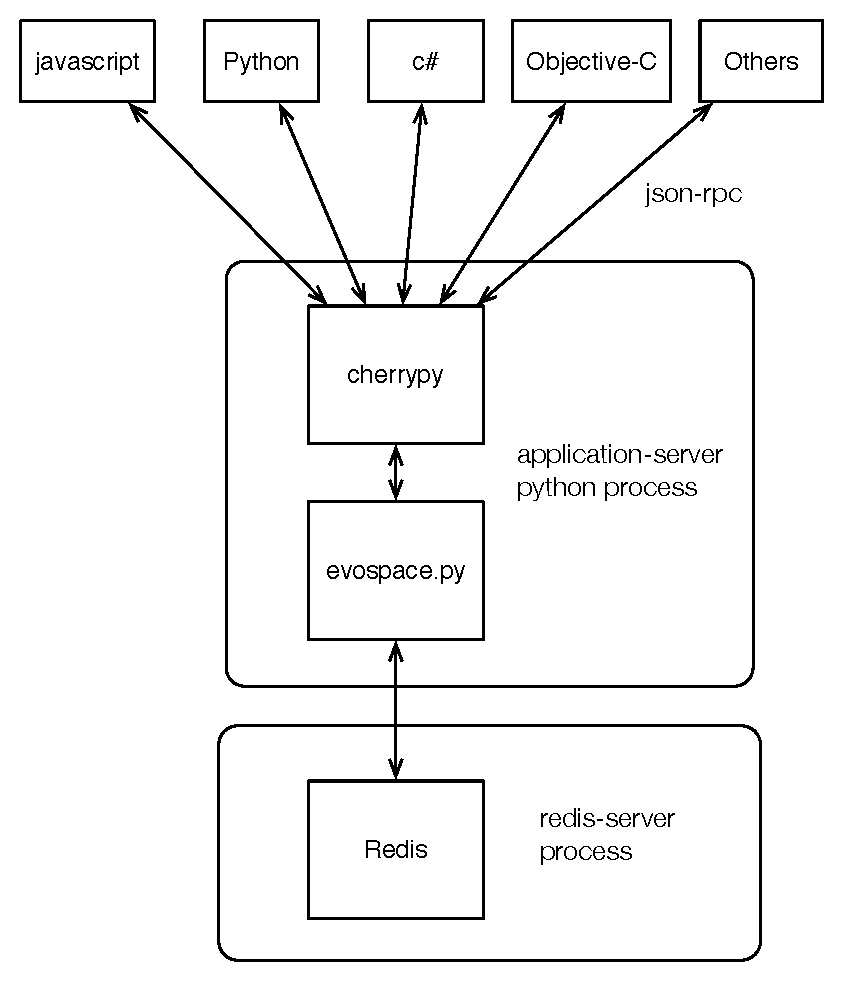
\includegraphics[width=8cm]{evospace.eps}
    \caption{EvoSpace-py implementation architecture } %EvoSpace the
                                %whole enchilada? EvoSpace the
                                %population store? Why implementation
                                %in Capitals? - JJ
    \label{fig:evospace}
\end{figure*}

On the other hand, EvoWorkers must implement the genetic operators for a particular EA.
Given that EvoSpace-py is implemented as a Python module, a simple way to implement EvoWorkers is by using the basic non-distributed GA found in the Distributed Evolutionary Algorithms in Python (DEAP) library \cite{DEAP_JMLR2012}. 
However, three methods were added to the local DEAP algorithm: $getSample()$ and  $setSample()$; and  another for the  initialization of the population using DEAP´s own methods.
For instance, to generate the initial population DEAP's $initialize()$ method  is called and the generated population is sent to EvoSpace, then for each generation $getSample()$ function is called, this executes the EvoStore $Take()$ method, and the received sample is used to create a DEAP population which is then evolved for a predefined number of generations.
Finally, the $setSample()$ function converts the DEAP population to a JSON object and returns it to the EvoStore through the $Replace()$ method.   

\subsection{EvoSpace-py in a Cloud Architecture}
The first version of EvoSpace-py was implemented as a multi-process application running in a single computer, this implementation was used to run the first set of experiments described in Section \ref{sec:exp1}.
However, a networked based implementation was needed to further evaluate the ESM.  
This section describes how EvoSpace-py can be configured to run on a cloud architecture using two Platform as a Service (PaaS) components, Heroku for the EvoSpace Server and PiCloud for simulating EvoWorkers; a schematic view of the cloud architecture is shown in Figure~\ref{herokuPiCloud}.

\begin{figure}[t]
\centering
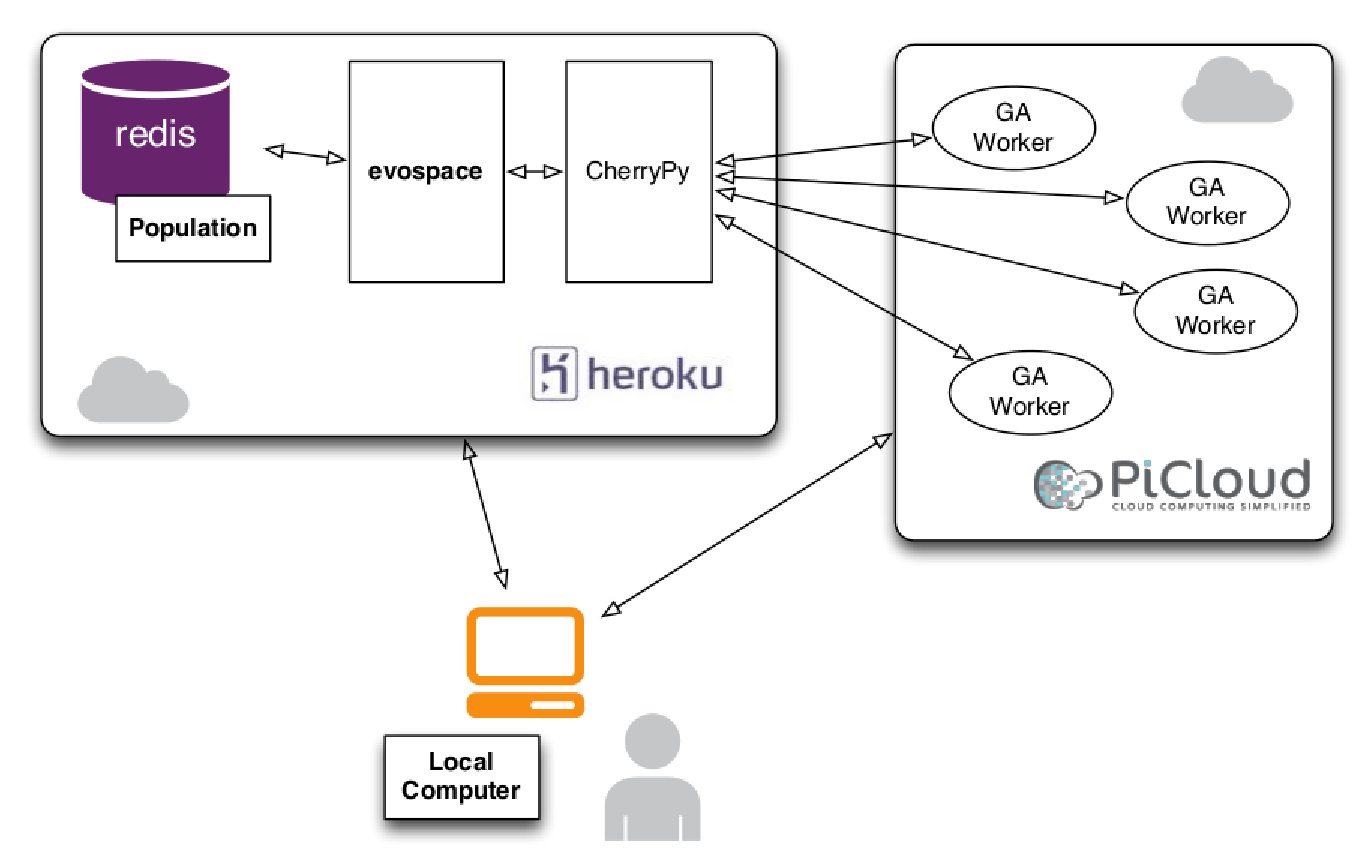
\includegraphics[width=3.2in]{herokuPiCloud.eps}
\caption{EvoSpace-py cloud-based architecture.}
\label{herokuPiCloud}
\end{figure}

Heroku (\url{http://heroku.com}) is a multi-language PaaS, supporting among others Ruby, Python and Java applications. The basic unit of composition on
Heroku is a lightweight container running a single user-specified
process. These containers, which they call {\em dynos}, can include web
(only these can receive {\tt HTTP} requests) and worker processes
(for instance processes used for database backups or task queues).
These  process types are the prototypes from which one or more dynos 
can be instantiated; if the number of requests to the server increases then 
more instances can be assigned on-the-fly. In our case, our CherryPy 
web application server runs in one web process, when the number 
of workers was increased we added more dynos (instances) of the 
CherryPy process. This model is very different from a Virtual Private Server (VPS) where users pay for the whole server; in a process based model, users pay only for the processes they need; being a {\em freemium} model means also that, if a minimum level of resources is not exceeded, it can be used for
free. 
Once deployed the web process can be scaled up by assigning more dynos;
for instance, in the more demanding experiments the web process was scaled to 20 dynos.
%Instructions and code for deployment is available at \url{http://www.evospace.org/software.html} 


\subsection{EvoWorkers as PiCloud Jobs}
PiCloud is a PaaS, with deep Python integration, such that functions are transparently uploaded to PiCLoud's 
servers as units of computational work they call jobs. 
Each job is added to a queue, and when there is a computing core available, 
the job is assigned to it. Both Heroku and PiCloud 
platforms are deployed on top of the Amazon Web Services (AWS) 
infrastructure in the US-EAST Region. This ensures minimal 
latency and a high bandwidth communication between the services, 
and there is no charge for data transfer costs between both services.
%For the experiments type c1 and c2 Real Time workers where used.  
%The code for the EvoWorkers implementation and experiment data is publicly available from a Github repository \url{https://github.com/mariosky/evoPar2014}. 
% \url{http://goo.gl/92tMFw}. % Github tiene su
                                % propio acortador, pero también
                                % tienes que anonimizarlo - JJ 

%The following sections present an experimental evaluation of the ESM through the reference implementation (evospace-py) using standard benchmark problems for GAs.
%In particular, EvoSpace is first evaluated based on performance and efficiency, compared to a canonical GA, this is done
%in Section \ref{sec:exp1}.
%Afterwards, specific issues with Pool-EA algorithms are discussed and experimentally evaluated in Section \ref{sec:overcome},
%that illustrate how potential shortcomings are avoided with the EvoSpace framework.


\section{Experiments and Results}
\label{sec:exp1}
The goal of this section is to evaluate the ESM and the proposed EvoSpace-py implementation, using well-known benchmarks for GAs,
the OneMax problem, the K-trap problem \cite{trap} and the P-Peaks problem \cite{Jong:PS97}.
In particular, two different versions of EvoSpace-py are evaluated, a local multi-process implementation and a cloud-based implementation,
using three experimental setups.
In the first experiment, the ESM is compared with the IMEA using the OneMax problem, to evaluate how it compares to a closely related EA model that is also
amenable to distributed computing frameworks.
In the second experiment, the ESM is evaluated based on its ability to find local optima on the deceptive K-trap problem,
comparing its performance and diversity with that of a canonical GA.
Finally, in the third experimental setup the speedup offered by the cloud-based implementation is evaluated given the communication overhead
that the distributed approach requires, comparing it with a local execution.
 %To prove what? Validate the approach? Check
                  %performance? Scalability? Both? - JJ


\subsection{Experiment A: Comparison with IMEA using OneMax}
These experiments focus on comparing EvoSpace with an IMEA using the classic OneMax problem.
In particular, the goal is to evaluate search efficiency and the computational effort of each of these strategies.
To do so, a 128-bit OneMax problem is chosen, using a binary-coded GA with one point mutation and two point crossover.
The population is set to the minimum size that guarantees that
a solution will be found in over 90\% of the runs following the strategy described in \cite{nodeo},
additional configuration details are given in Table \ref{tab:exp3}.
%In the case of SofEA results are taken from those published in \cite{sofea3}, where a multi-processor local implementation is used.
EvoSpace and the IMEA are executed locally, for the latter the reference implementation provided by DEAP is used.
For EvoSpace, the problem is tested with 2,3,4 and 6 distributed workers,
and for the IMEA the same number of demes, or islands, are used. In each case, a different population (or deme) size is used, or in 
the case of EvoSpace a different sample size, following \cite{nodeo}.

Figure \ref{fig:island} presents a comparison based on the total number of fitness function evaluations required to find a solution
and the total time to solution.
Figures \ref{fig:island}(a) and \ref{fig:island}(b) show the total number of evaluations for EvoSpace and IMEA respectively,
and Figures \ref{fig:island}(c) and \ref{fig:island}(d)  show the same for total time to solution.
First, it is clearly shown that EvoSpace performs a more efficient search that the IMEA, requiring about half the total number of fitness evaluations 
in all cases. Moreover, with EvoSpace the number of fitness evaluations seems to be independent of the number of workers that participate in the search, in all cases the median number of evaluations is below 20K.
On the other hand, the IMEA shows greater variability, with median values varying from around 35k to as much as 50k depending on the number of
demes, without a clear trend.

On the other hand, regarding time to solution, it seems clear that with more workers EvoSpace performs better, with median results of 2.3s with 2 workers down to 1.5 with six workers.
The IMEA, however, varies between 0.7s and 1.1s, without any clear improvement as the number of demes increases.
These results are expected, given that the IMEA is executed within the same DEAP process, while EvoSpace is incurring a communication overhead between Redis, JSON and DEAP.
However, in a distributed network such overheads would be unavoidable for any model, and in real-world scenarios fitness evaluations tend to be the most severe bottleneck.
Therefore, these results suggest that EvoSpace can perform a more efficient search process that an IMEA.


\begin{figure*}[t]
    \centering
    \subfigure[EvoSpace]
    {
       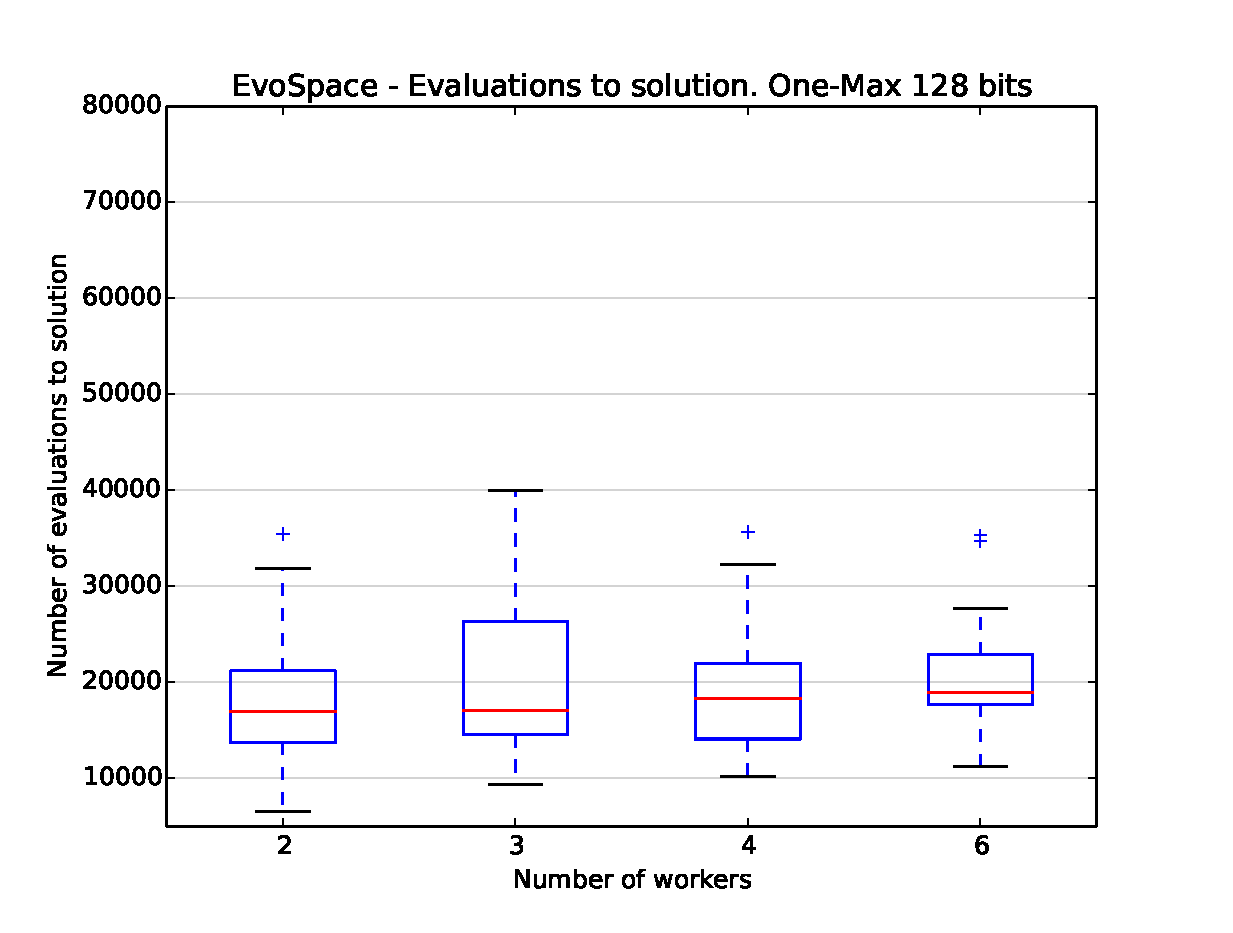
\includegraphics[width=5.9cm]{one_max_plot_evaluations_evospace.eps}
       %\includegraphics[width=5cm]{Plot-Individuals-Eval-k4w32s32.eps}

    }
    \subfigure[IMEA]
    {
        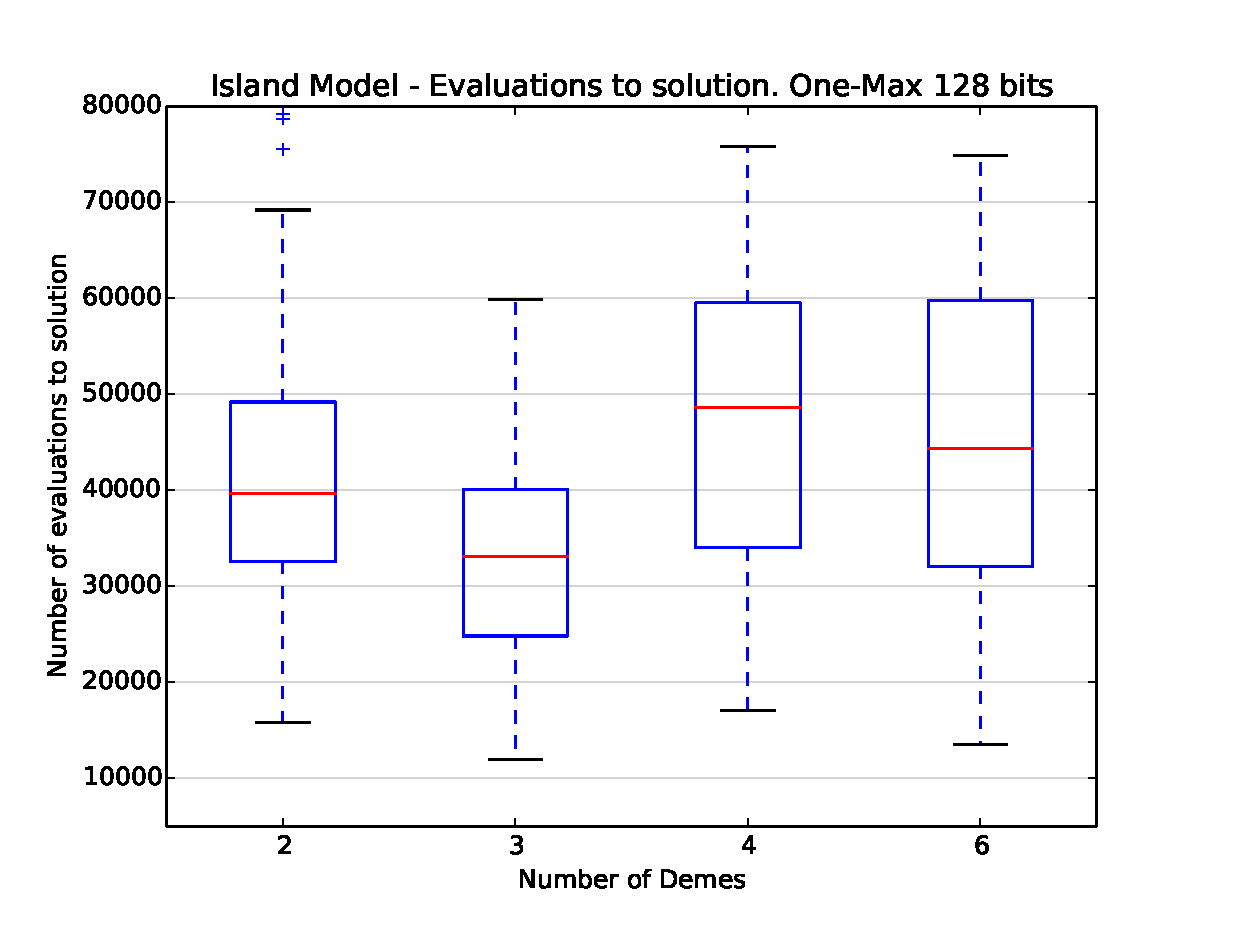
\includegraphics[width=5.9cm]{one_max_plot_evaluations_island.eps}
    }
    \\
    \subfigure[EvoSpace]
    {
        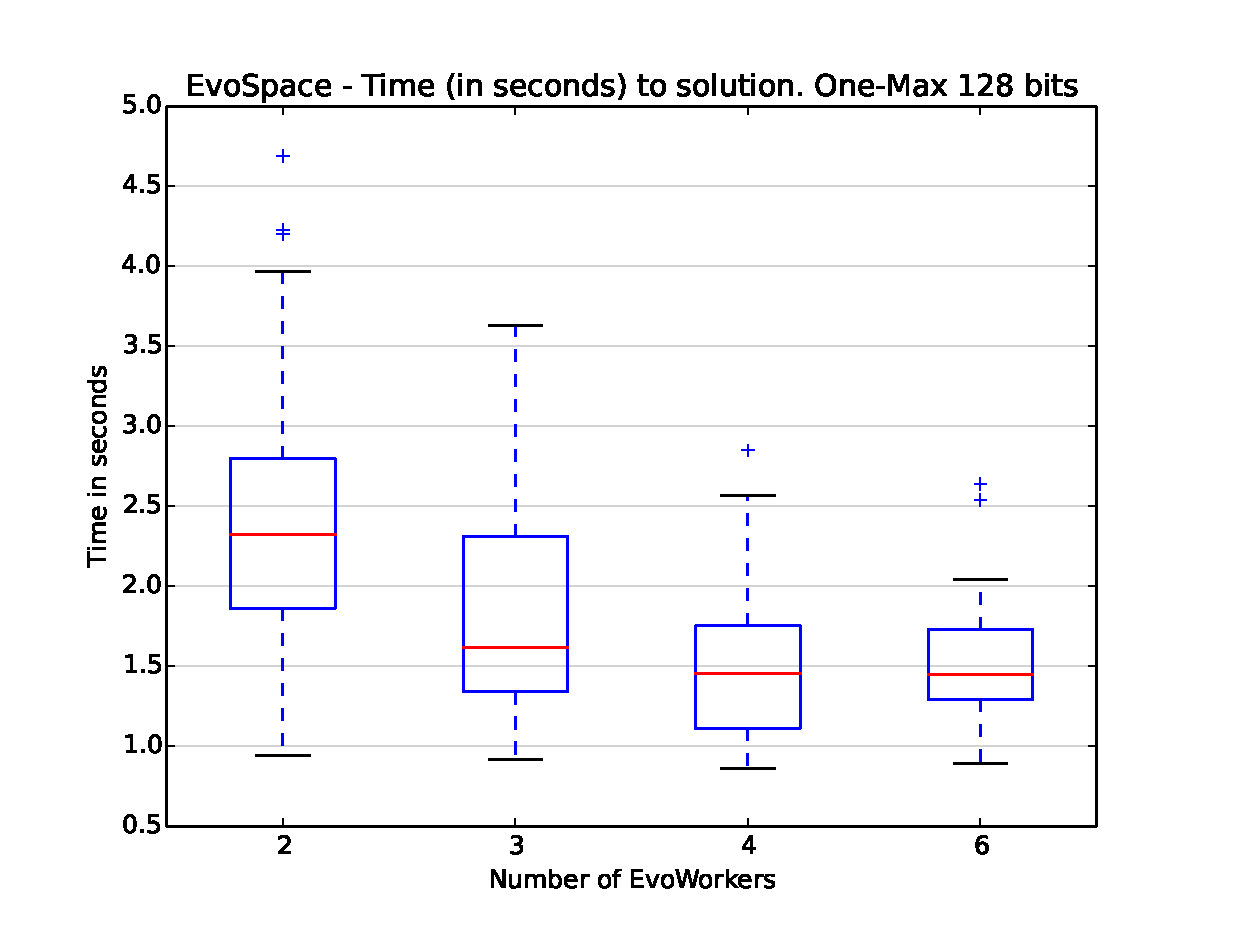
\includegraphics[width=5.9cm]{one_max_plot_time_evospace.eps}
    }
    \subfigure[IMEA]
    {
        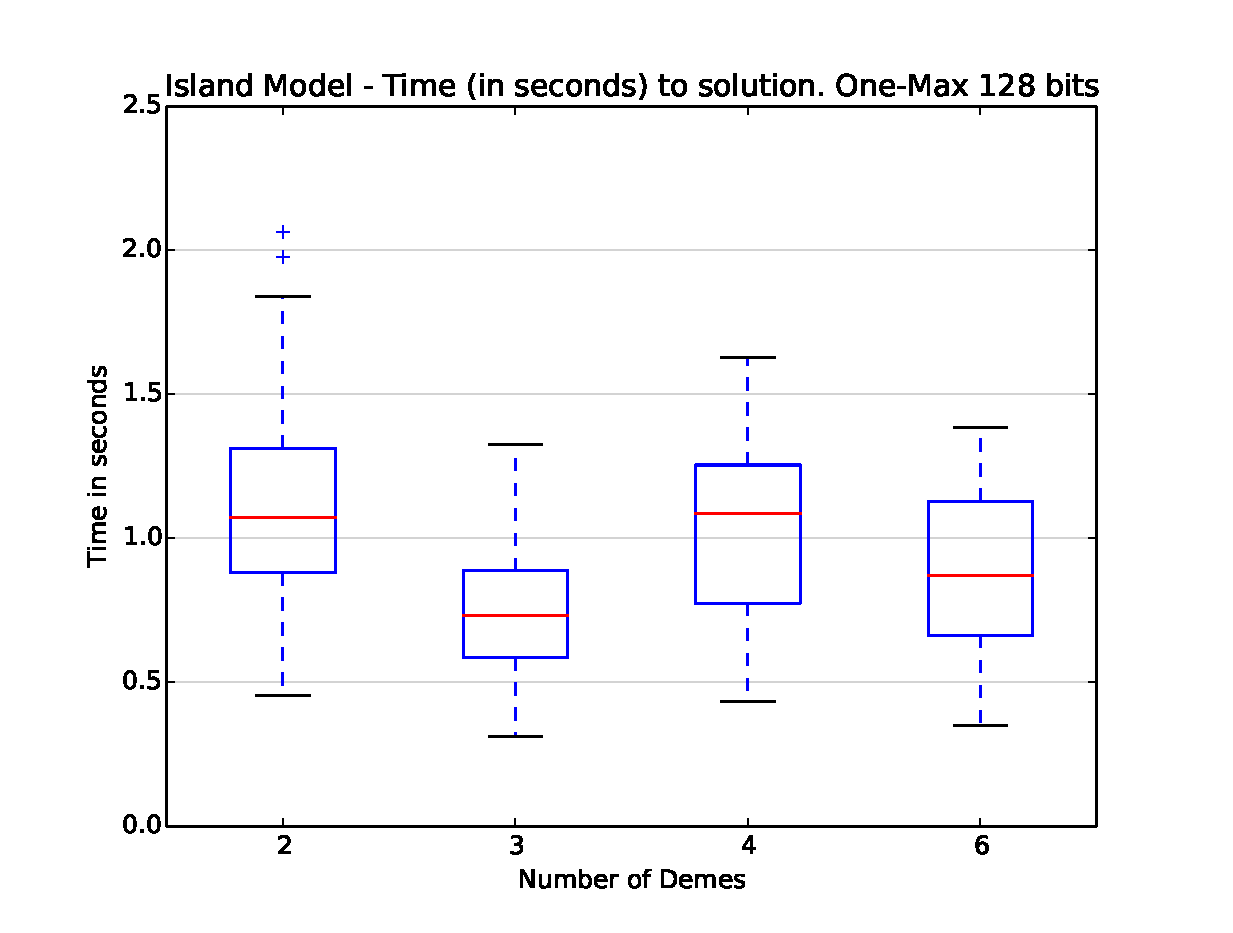
\includegraphics[width=5.9cm]{one_max_plot_time_island.eps}
    }
    \caption{
    Comparison of EvoSpace with an IMEA: (a,b) Number of fitness function evaluations; (c,d) Total time to solution.}
    \label{fig:island}
\end{figure*}


\begin{table}[t]
\renewcommand{\arraystretch}{1.3}
\caption{Parameters for EvoSpace and the IMEA on the OneMax problem.}
\label{tab:exp3}
\centering
\begin{tabular}{|l||c|}
\hline
\multicolumn{2}{|c|}{EvoSpace} \\
\hline
Population size & 64,64,64,52 \\
Sample Size & 24,18,12,8 \\
Worker generations & 30 \\
\hline
\multicolumn{2}{|c|}{IMEA} \\
\hline
Deme size & 80,40,38,25 \\
Generations & 30 \\
Migration rate & 5 \\
\hline
\multicolumn{2}{|c|}{Shared Parameters} \\
\hline
Crossover prob. & 0.5 \\
Mutation prob.  & 0.2 \\
Tournament selection & size 4 \\
\hline
\end{tabular}
\end{table}


\subsection{Experiment B: K-trap Function}
For these experiments the K-trap function is used to test the ESM, a problem that presents a multi-modal and deceptive fitness landscape.
Table \ref{tab:exp} summarizes the different experimental configurations tested, based on the $K$ value, number of EvoWorkers, the sample size taken by each worker and the chromosome length.
A bit-string representation is used, and each EvoWorker performs 100 total generations on each sample,
using one-point crossover (with crossover probability set to 1) and one-point mutation (mutation probability set to 0.06).
The number of individuals in the EvoStore is set to 1024 for 4-trap experiments and to 4096 for 5-trap,
and the maximum number of total samples that can be taken from the EvoStore in each run is set to 1000.
For comparison, a standard GA is applied to each benchmark problem.
For the 4-trap problem the maximum number of generations is set to 4000, and for the 5-trap problem it is set to 1000.
These values limit the maximum number of function evaluations that can be performed, in fact these values were chosen so the limit is equivalent to the
maximum number of function evaluations from all of the EvoSpace runs; however, most EvoSpace runs required much less function evaluations than these maximum values.
In total, $50$ runs were performed for each experimental configuration.


\begin{figure*}[t]
    \centering
    \subfigure[Evolution of Fitness]
    {
       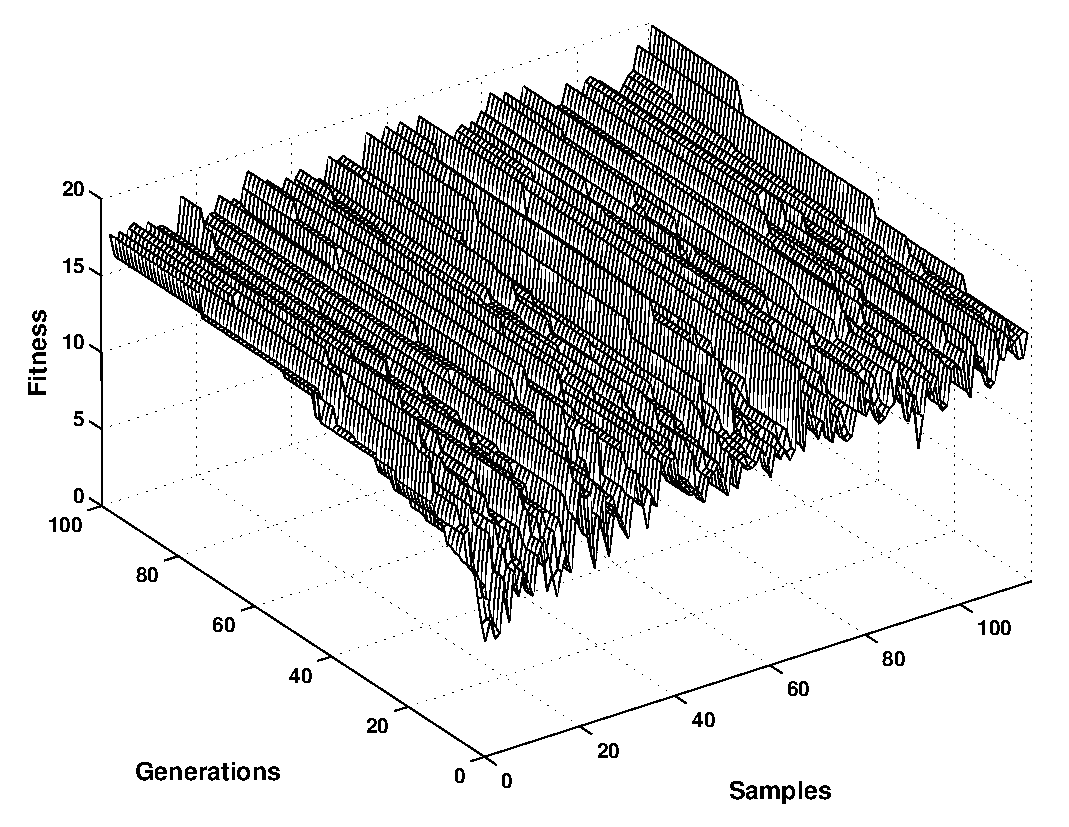
\includegraphics[width=5.9cm]{Plot-Surface-Best-Run0-k5w4s64.eps}
       %\includegraphics[width=5cm]{Plot-Individuals-Eval-k4w32s32.eps}

    }
    \subfigure[Evaluated]
    {
        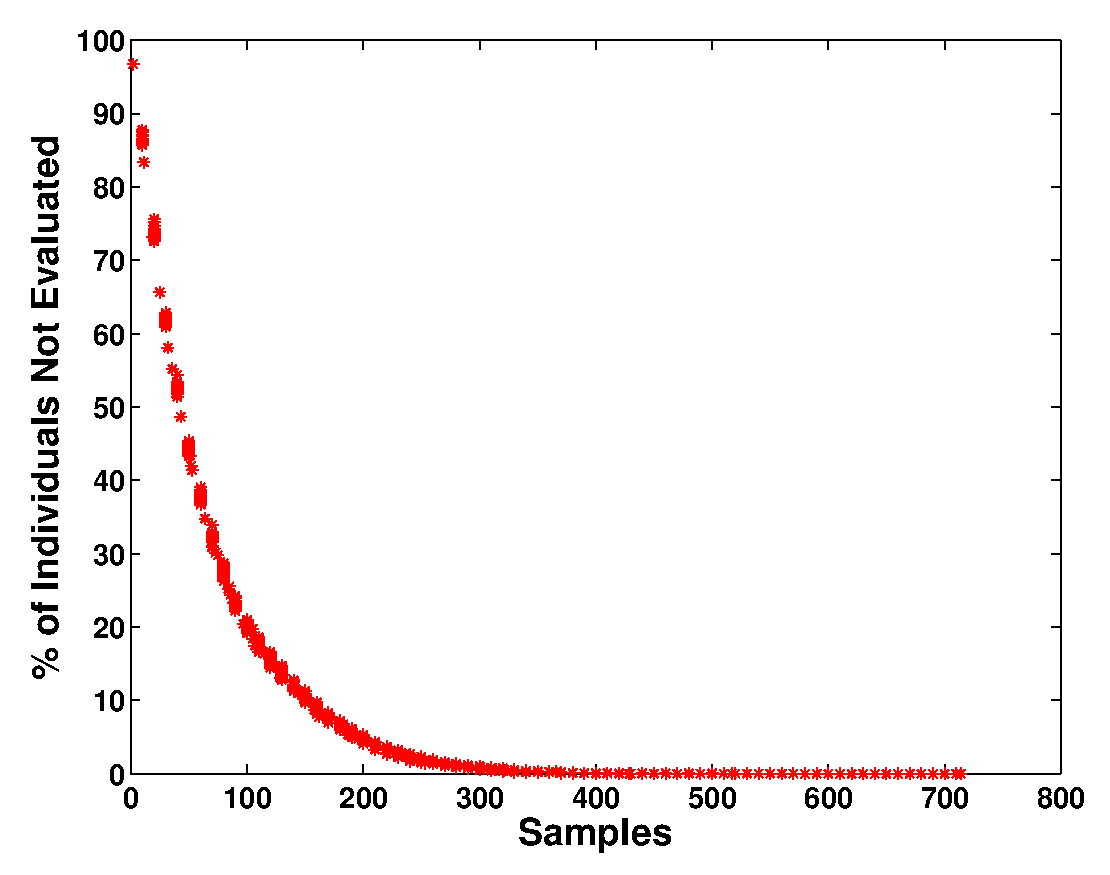
\includegraphics[width=5.9cm]{Plot-Individuals-Eval-k5w4s64.eps}
    }
    \\
    \subfigure[EvoSpace]
    {
        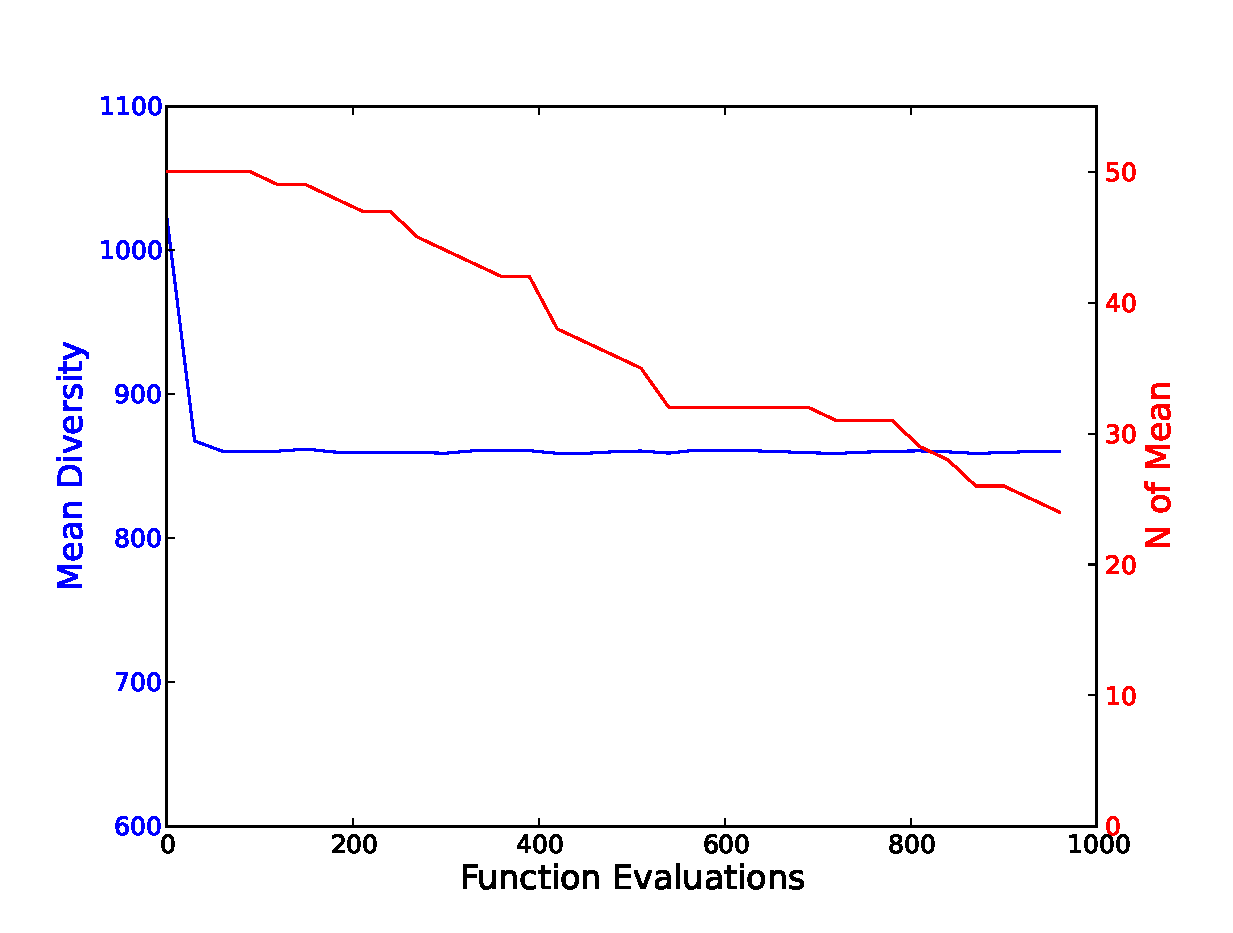
\includegraphics[width=5.9cm]{DivMeanEvoSameScale.eps}
    }
    \subfigure[Standard GA]
    {
        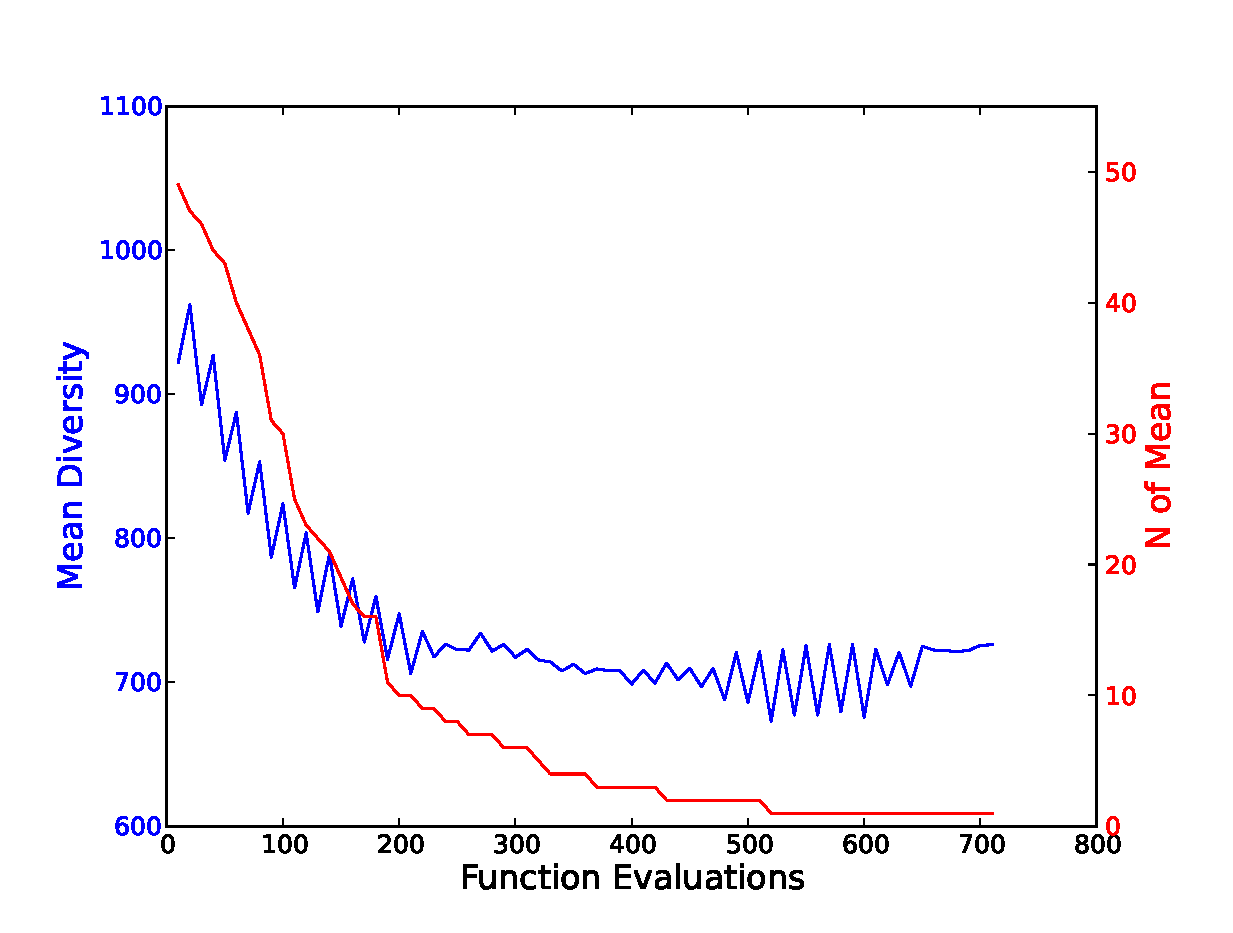
\includegraphics[width=5.9cm]{DivMeanGASameScale.eps}
    }
    \caption{
    These plots summarize the results for Experiment K:
    (a) evolution of fitness for a single run, the plot shows how fitness evolves for each sample taken by the EvoWorkers;
    (b) scatter plot, considering all runs, of the percentage of non-evaluated individuals;
    (c-d) evolution of diversity, these are y-axis plots that show the mean diversity over all runs (dark line) and the number of runs $N$ used to compute the mean.}
    \label{fig:others}
\end{figure*}

Figure \ref{fig:others}a depicts how fitness evolves over all of the samples taken from EvoSpace.
This figure shows the evolution of best-fitness for a single run of experiment K in Table \ref{tab:exp};
the analysis focuses on a single run instead of the mean of all runs to emphasize the local dynamics of the evolutionary process.
The plot shows how fitness evolved on each EvoWorker that participated in the search.
Evolution of fitness is organized based on the two temporal axis of the horizontal plane,
one corresponds with the sample number, independent of which EvoWorker took the sample, and the other corresponds
to the generations of the local evolutionary process executed on the EvoWorker.
In other words, these plots provide a collective view of the evolutionary process from the perspective of all EvoWorkers.
Since the global optimum is a fitness value of 10, we can see that the evolution on the last sample taken from EvoSpace reaches the global optimum;
also notice the low fitness value for the first few samples taken in the initial generations.

%and after this no more samples are taken since the search is halted at that moment.
%The overall performance of EvoSpace is summarized in Table \ref{tab:found}, which shows the total number of runs, out of $50$,
%that found the global optima.
EvoSpace outperforms the standard GA on both tests, with a substantial increase in the number of optima found.
In eleven experiments EvoSpace found the optimal solution in all runs, in the other four cases (experiment A,D,E and H) it does no worse than
48 total optima found.
On the other hand, the sequential GA only finds 34 optima on the 5-trap problem and 29 on the 4-trap case.
These results were not expected, since the EvoSpace algorithm is using the same representation and search operators (mutation and crossover) than the standard
GA. Therefore, it is evident that the novel population dynamics induced by the ESM model are able to substantially improve the quality of the results
while otherwise using a basic representation and genetic operators.

\begin{table}[t]
\caption{Different experimental configurations used to test the
  performance of EvoSpace.} %Why these? What do you want to evaluate?
                            %Is it complete? 
\centering
\scriptsize
\begin{tabular}{|l||c|c|c|c|c|c|c|c|c|c|c|c|c|c|c|}
   \hline
             \textbf{Experiment} 	& A & B & C & D & E & F & G & H & I & J & K & L & M & N & O \\

   \hline
               \textbf{K-trap}   	& 4  & 4  & 4  & 4  & 4  & 4  & 4  & 4  & 4 & 5 & 5 & 5 & 5 & 5 & 5 \\
			   \textbf{EvoWorkers}  & 1  & 1  & 4  & 4  & 8  & 8  & 16 & 16 & 32 & 1 & 4 & 8 & 16 & 32 & 40 \\
			   \textbf{Sample size} & 32 & 64 & 32 & 64 & 32 & 64 & 32 & 64 & 32 & 64 & 64 & 64 & 64 & 64 & 64 \\
			   \textbf{Chromosome} & 40 & 40 & 40 & 40 & 40 & 40 & 40 & 40 & 40 & 50 & 50 & 50 & 50 & 50 & 50 \\
   \hline
\end{tabular}
\label{tab:exp}
\end{table}


%\begin{table}[t]
%\caption{Parameters and algorithm configurations for all experiments.}
%\centering
%\begin{tabular}{|c||c|c|c|c|}
%   \hline
%                       & Maximum          &                    &                  & Generations per \\
%   \textbf{Parameter}  & total samples    & Crossover (Prob.)  & Mutation (Prob.) & EvoWorker        \\
%
%	\hline
%   \textbf{Value}     &	1000 &	Single point (1) &	Point  (0.06)   & 100    \\
%   \hline
%
%\end{tabular}
%\label{tab:exp2}
%\end{table}


%\begin{table}[t]
%\caption{Different experimental configurations used to test the performance of EvoSpace.
%GA-K are the baseline GA results for the 4-trap and 5-trap functions respectively.}
%\centering
%\tiny
%\begin{tabular}{|l||c|c|c|c|c|c|c|c|c|c|c|c|c|c|c|c|c|}
%   \hline
%             \textbf{Experiment} & A & B & C & D & E & F & G & H & I & J & K & L & M & N & O & GA-4 & GA-5 \\
%
%   \hline
%        \textbf{Optima found}   & 48 & 50 & 50 & 49 & 49 & 50 & 48 & 50 & 50 & 50 & 50 & 50 & 50 & 50 & 50 & 34 & 29 \\
%
%   \hline
%\end{tabular}
%\label{tab:found}
%\end{table}

\begin{figure*}[t]
    \centering
    \subfigure[]
    {
        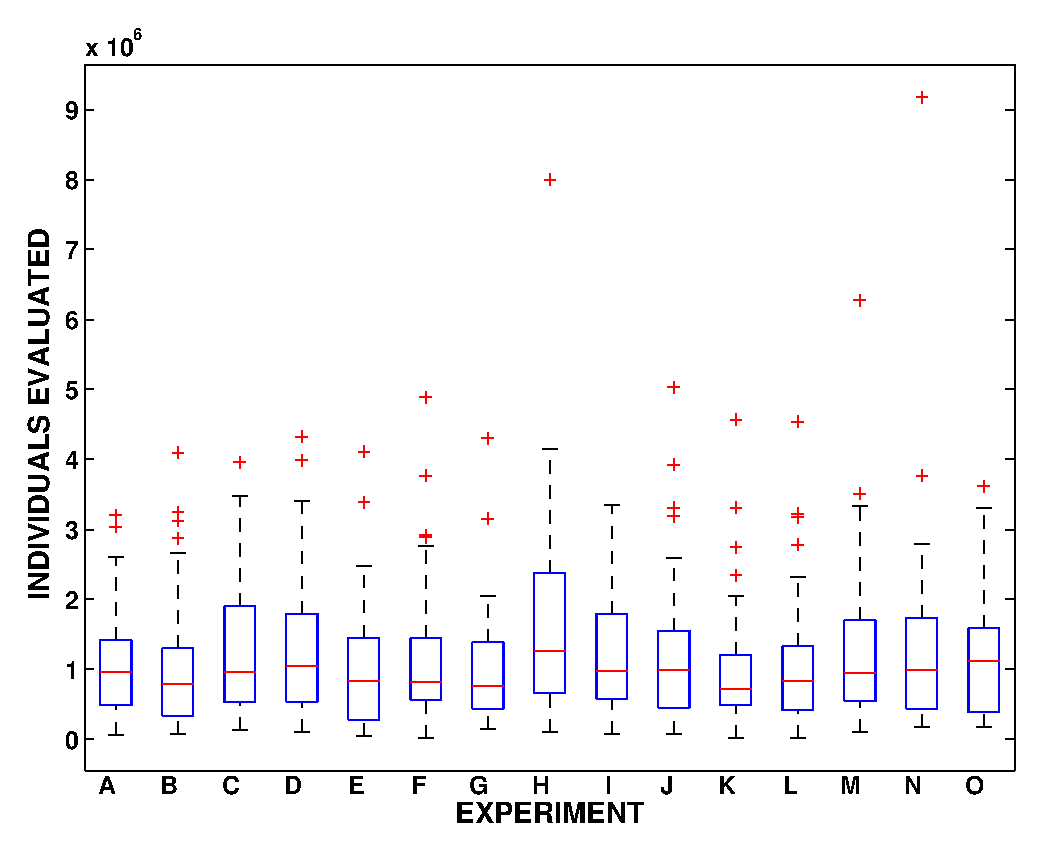
\includegraphics[width=5.9cm]{Evaluados.eps}
    }
    \subfigure[]
    {
        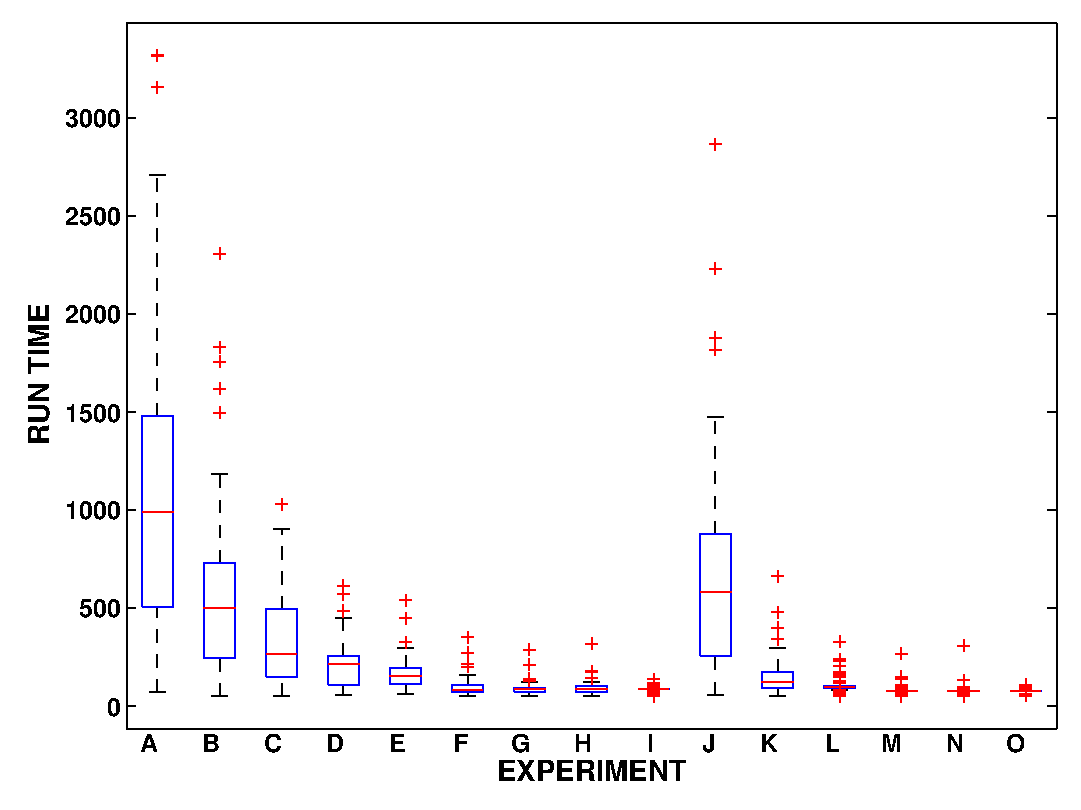
\includegraphics[width=5.9cm]{TimeBox.eps}
    }
    \caption{
    (a) Number of evaluated individuals over all runs.
    (b) Total run-time.}
    \label{fig:effort}
\end{figure*}

Since every EvoWorker takes a random sample of individuals, one concern might be that some individuals of the initial population might
not be chosen and evaluated wasting valuable genetic material.
Figure \ref{fig:others}b shows a scatter plot of all of the runs for experiment K, depicting the percentage of individuals
that have not yet been evaluated; here it is important to remember that some runs required more samples than others.
The figure clearly shows that the percentage individuals not evaluated within EvoSpace quickly decreases as more samples are taken.
Another interesting question is how the EvoSpace search impacts diversity, here given by the sum of the pairwise Hamming distances
of all individuals within the population \cite{diversity}.
Figure \ref{fig:others}c shows how diversity evolves for experiment K, and
Figure \ref{fig:others}d shows the same for the basic GA\footnote{The time scale is given by
the number of individuals evaluated, increments correspond to the number of individuals evaluated in 10 samples.}.
These plots show how the standard GA has a problem maintaining diversity, which leads to its poor performance.
On the other hand, EvoSpace maintains a more diverse population which leads to a better exploration of the search space and more successful runs.

Finally, a comparison of the computational effort required in each experiment is given in
Figure \ref{fig:effort}, which shows boxplots of all runs in each experiment.
Figure \ref{fig:effort}a plots the total number of individuals evaluated in each run, which is similar in all experiments
and consistent with the results from Experiment A;
while Figure \ref{fig:effort}b compares the total run time in seconds.
Figures show that run time is significantly reduced as the number of EvoWorkers increases.



\subsection{Experiment C: P-Peaks}
\label{expb}
% Why this second experiment? Do you want to prove something you
% haven't before?  - JJ 

The P-Peaks problem was chosen because the problem and consequently the computing resources needed for the search can be appropriately scaled.
Proposed by De Jong et al. in \cite{Jong:PS97}, as a generalization of the version in \cite{Jong:1990}, a
P-Peaks instance is created by generating a set of P random N-bit
strings, which represent the location of the P peaks in the space. To
evaluate an arbitrary bit string \begin{math} \mathbf{x} \end{math}
first locate the nearest peak (in Hamming space). Then the fitness of
the bit string is the number of bits the string has in common with
that nearest peak, divided by N. The optimum fitness for an individual
is 1, and is computed by

\begin{equation}
f_{P-PEAKS}(\mathbf{x})=\frac{1}{N} \overset{P}{\max_{i=1}} \{N-hamming(\mathbf{x},Peak_i)   \} \ .
\end{equation}

A large number of peaks induces a time-consuming search,
since evaluating every string is computationally expensive; this is
convenient since in order to justify a distributed EA fitness computation has to be significantly larger than the associated
network latency (otherwise, it would always be faster to have a single-processor version).
For this work, the experiment is setup with $P = 256$ peaks and $N = 512$ bits, a configuration that requires considerable computational time for
fitness evaluation, and 30 runs are performed.
Regarding algorithm parameters these are summarized in Table \ref{tab:paramse},
in particular notice that these experiments use c1 Real Time workers, which are highly efficient cpu's.

\begin{table}[t]
\renewcommand{\arraystretch}{1.3}
\caption{GA and EvoWorker parameters for Experiment C.}
\label{tab:paramse}
\centering
\begin{tabular}{|l||c|}
\hline
\multicolumn{2}{|c|}{GA Parameters} \\
\hline
Tournament size & 4 \\
Crossover rate & 0.85  \\
Population Size & 512 \\
Mutation probability & 0.5 \\
Independent bit flip probability  & 0.02 \\
\hline
\multicolumn{2}{|c|}{EvoWorker Parameters} \\
\hline
Sample Size & 16 \\
Generations & 128 \\
\hline
\multicolumn{2}{|c|}{Variable Parameters} \\
\hline
PiCloud Worker Type & c1 Realtime, c2 Unreliable Realtime \\
Number of Workers & 2,4,8,16,28 \\
Number of Executions & 30 \\
\hline

\end{tabular}
\end{table}

As a baseline execution, the experiment was also conducted on a local computer. The specifications for the local computer are as follows, a
2.2 Ghz Intel Core i7 processor, 16 GB of 1333 DDR3 memory, and Mac OS X 10.7.5,
using the Python interpreter version 2.7.2 for 64-bit architectures. 
In this setting, the problem required considerable computational time: each run took an average of 1567.36 seconds to find the optimal solution.
The execution used a single core and CPU activity remained low for the whole length of the experiment. On the other hand,
the parallel execution time was significantly lower even when only two workers were used, clocking in at less than 180s even in the worst cases.

%\begin{table}[t]
%\renewcommand{\arraystretch}{1.3}
%\caption{Average Times and Evaluations of 30 executions in a local computer.}
%\label{local}
%\centering
%\begin{tabular}{|c|c|}
%\hline
%Average time in seconds & Average number of evaluations \\
%\hline
%1567.36 & 100690.5  \\
%\hline
%\end{tabular}
%\end{table}

Average times for the configuration using Realtime cores in PiCloud
are presented in Figure~\ref{fig:plot_time_real}. It can be seen that
incrementing the number of workers reduced the time to solution, but only up to 16 workers,
however with 28 workers the median time to solution did not improve.
There seems to be a point at which the overall speedup of the distributed search levels off in this experimental setup.
% This is
%related to the increase in the number of evaluations needed to find
%the optima, which is shown in Figure~\ref{fig:plot_evals_real}.
%This figure shows that the number of evaluations needed to find the
%solution increases as more workers are used. This behavior has an
%impact on the time to solution, because each evaluation (as stated
%earlier), is computationally expensive. From 2 to 8 workers the number
%of evaluations remains less than in the baseline GA, but from that point on
%the number is higher. A possible reason for this is that as
%the number of workers increases, the number of individuals that remain
%in the population waiting to be replaced decreases. As there are fewer
%individuals in the population the probability of taking the same individuals
%when replacing a sample is increased. This problem is also reported
%by Merelo et al. in  \cite{sofea:naco}, where they present a Pool-EA architecture with heterogeneous workers.

For problem domains where fitness evaluation of individuals is not demanding, the added overhead of communication between the EvoStore and the EvoWorkers
can become a concern.
However, our experiments suggest that this cost is practically negligible.
Figure~\ref{plot_ges} presents boxplots of the time required to perform the
three main EvoSpace-py functions on the EvoWorkers, computed over all of the 30 runs using 28 Realtime PiCloud workers.
It is clear that almost all of the computational time is consumed by the $Evolve()$ function which actually performs the search operations,
while the cost of taking a and returning a sample is relatively low.


\begin{figure*}[t]
    \centering
    \subfigure[Time to solution]
    {
        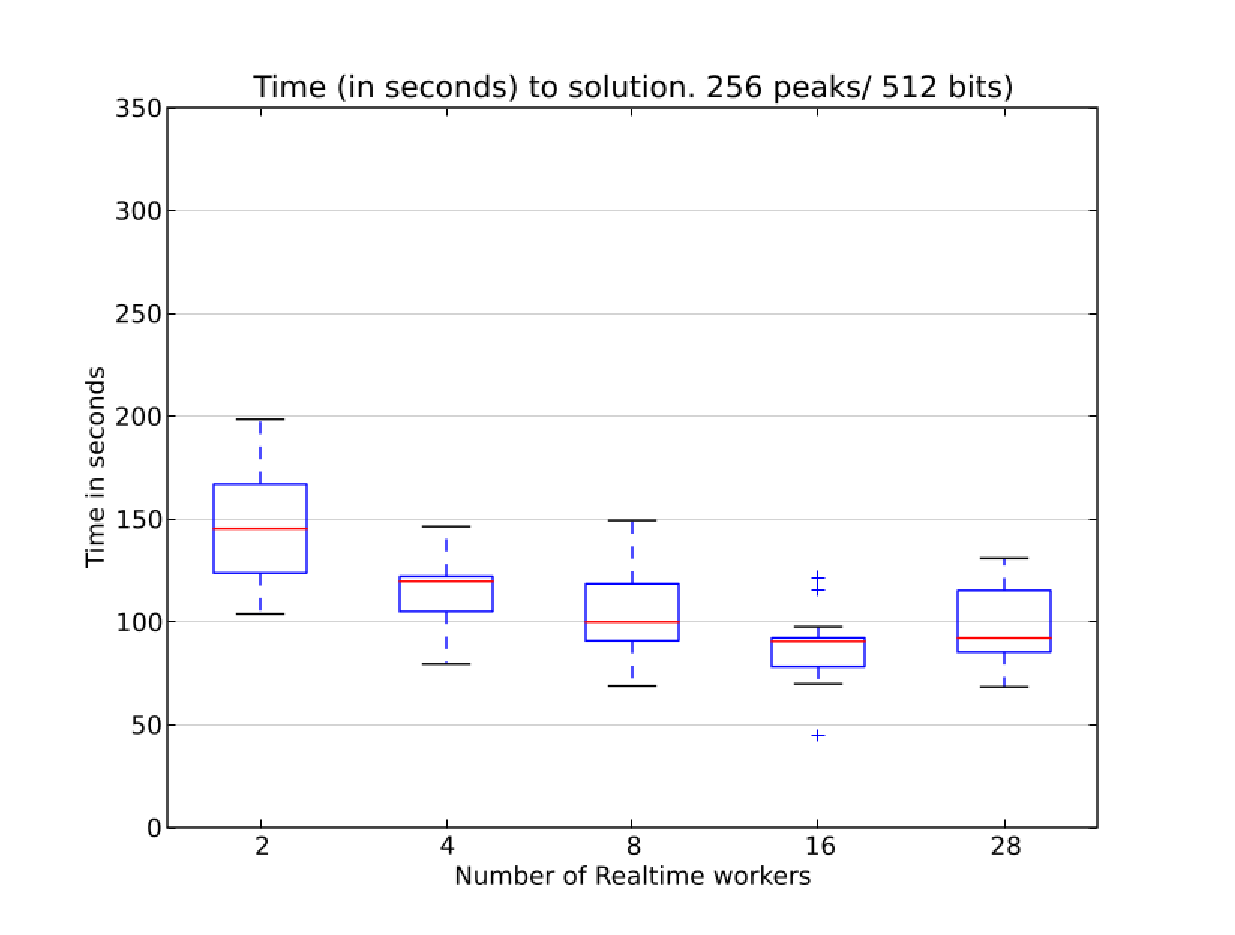
\includegraphics[width=5.9cm]{plot_time_realtime.eps}
        \label{fig:plot_time_real}
    }
%    \subfigure[Number of Evaluations]
%    {
%        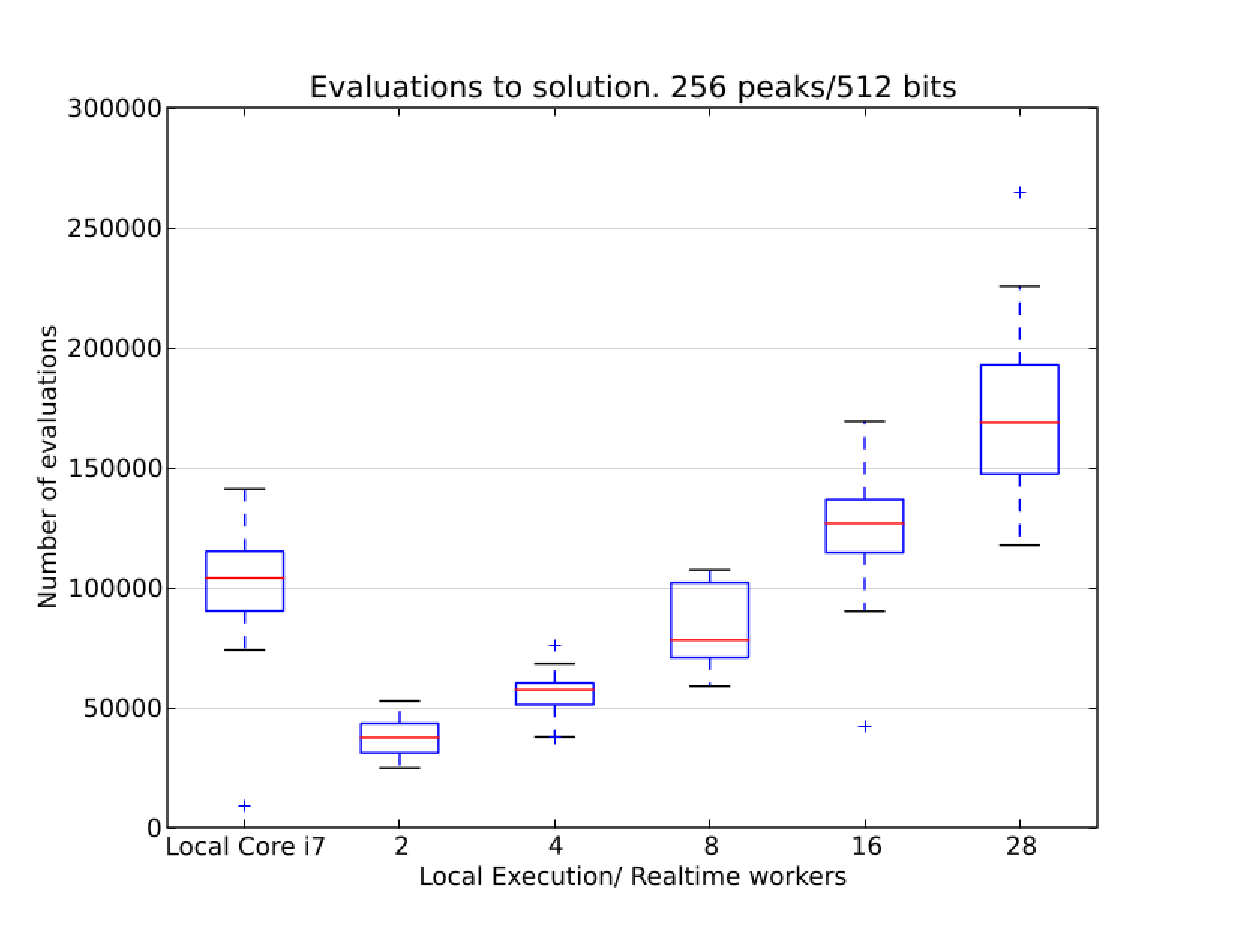
\includegraphics[width=5.9cm]{plot_evals_realtime.eps}
%        \label{fig:plot_evals_real}
%    }\\
        \subfigure[Worker Costs]
    {
        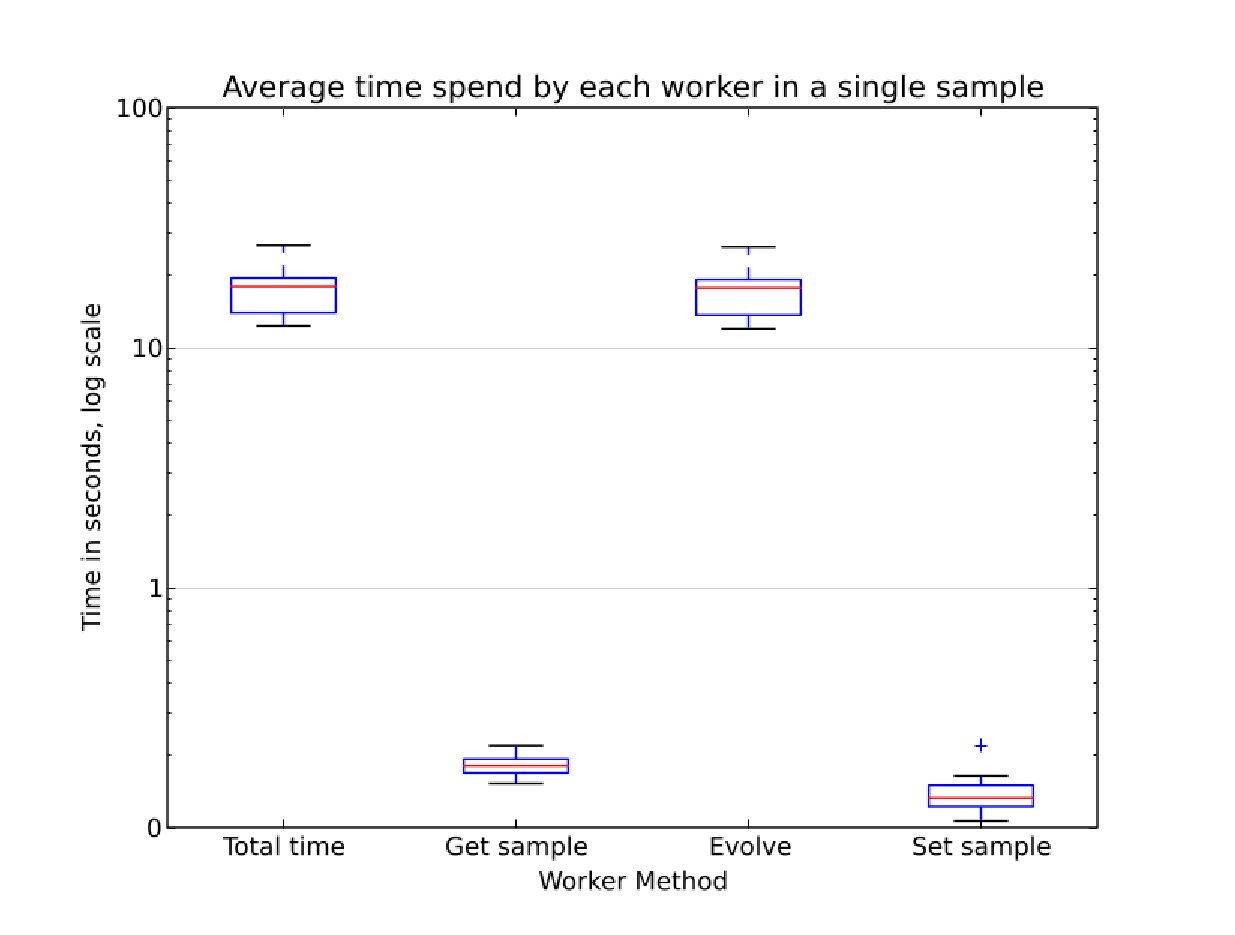
\includegraphics[width=5.9cm]{plot_ges.eps}
        \label{plot_ges}
    }
    \caption{Evaluation on the P-Peaks problem:
    (a) Time required to solution;
    (b) Number of evaluations to solution; (c) Time of worker's methods, getSample(), Evolve(), setSample().}
    \label{fig:effort_real_time}
\end{figure*}


%\subsection{Discussion}


\section{Overcoming Problems and Limitations}
\label{sec:overcome}
The previous section showed how the ESM can be used to implement a distributed and asynchronous Pool-EA based on the EvoSpace-py implementation,
with strong results.
However, as stated before, there are possible downsides to using a Pool-EA, some of which are directly addressed by the underlying ESM.
However, some issues persist, particularly the critical problem of possible lost work due to the unreliable connection of EvoWorkers,
and the tedious problem of algorithm parametrization, a common issue with almost all EAs that is severely amplified in a Pool-EA.

\subsection{Unreliable Workers}
In this section, the effect of node unavailability in an EvoSpace Pool-EA is assessed.
The ESM contrasts with the use of a global queue of tasks and implementations
of Map-Reduce algorithms, such as in \cite{fazenda2012}, with several benefits relevant to
concurrency control and workload distribution. 
%For instance, leaving a copy of the individual in the population server
%free to be pulled by other EvoWorkers will result in redundant work and this
%could be costly if the task at hand is time consuming.
EvoWorkers are expected to be unreliable, since they can loose a connection or could simply shut down or be removed from the client machine.
When an EvoWorker is lost, so are the individuals pulled from the population store.
Depending on the type of algorithm that is executed, the loss of these samples could have a high performance cost.
As stated before, to address this problem the ESM uses a reinsertion algorithm that also prevents
the starvation of the population pool. Other pool based algorithms normally use
a random insertion technique, but this might negatively impact the search process.

\begin{figure*}[t]
    \centering
    \subfigure[]
    {
        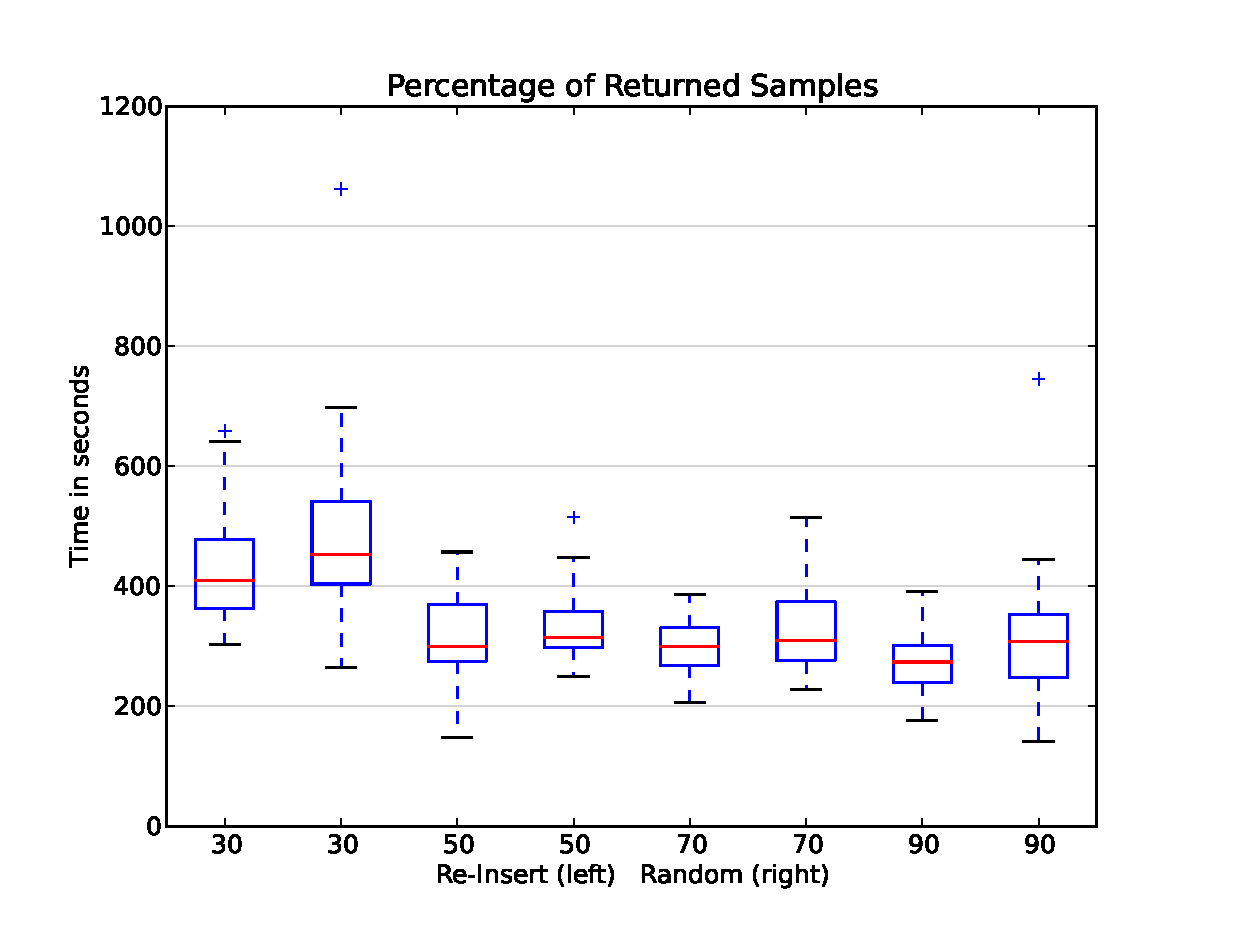
\includegraphics[width=5.9cm]{plot_time_CRS_w4.eps}
        \label{fig:plot_time_ri_w4}
    }
    \subfigure[]
    {
        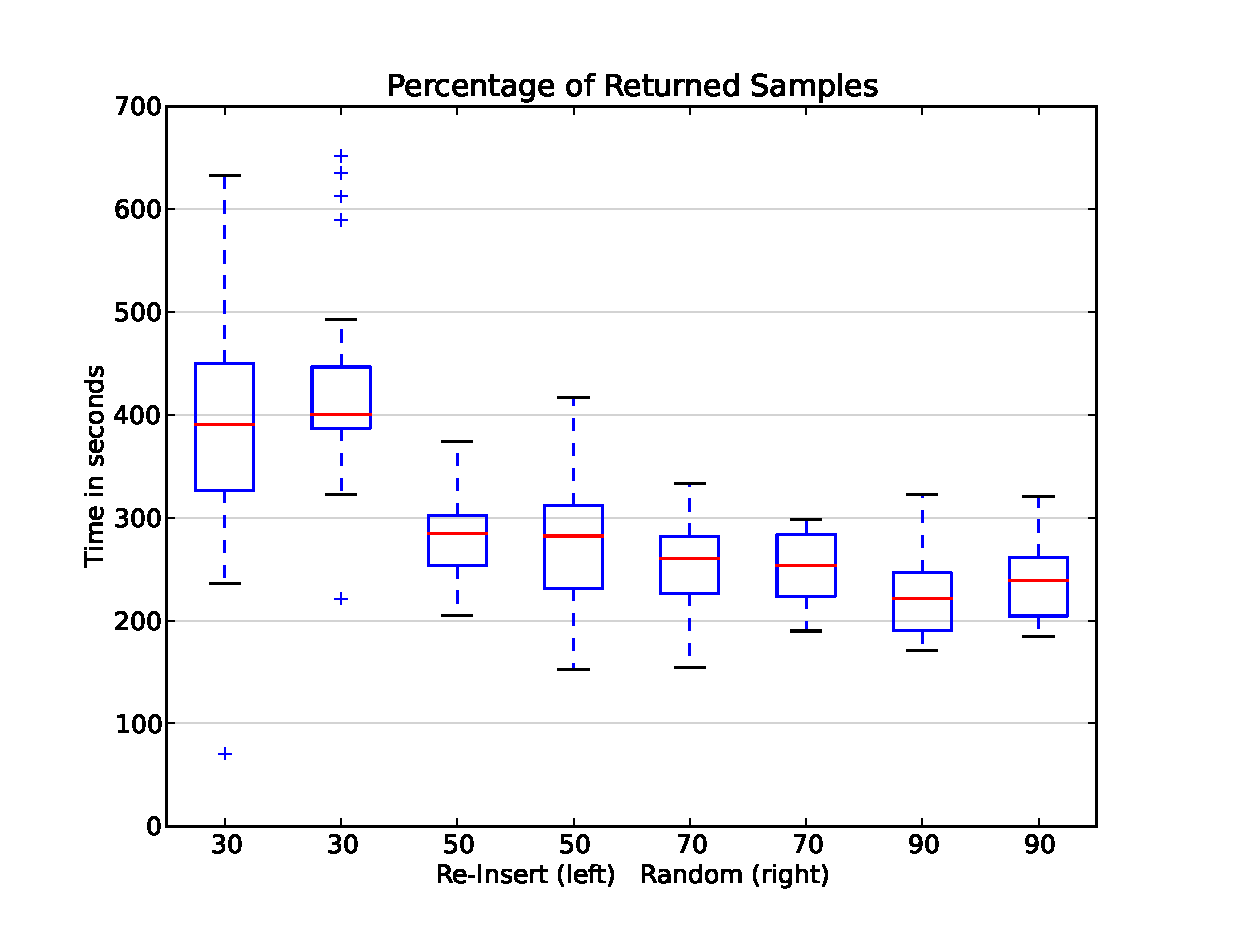
\includegraphics[width=5.9cm]{plot_time_CRS_w8.eps}
        \label{fig:plot_time_ri_w8}
    }
    \subfigure[]
    {
        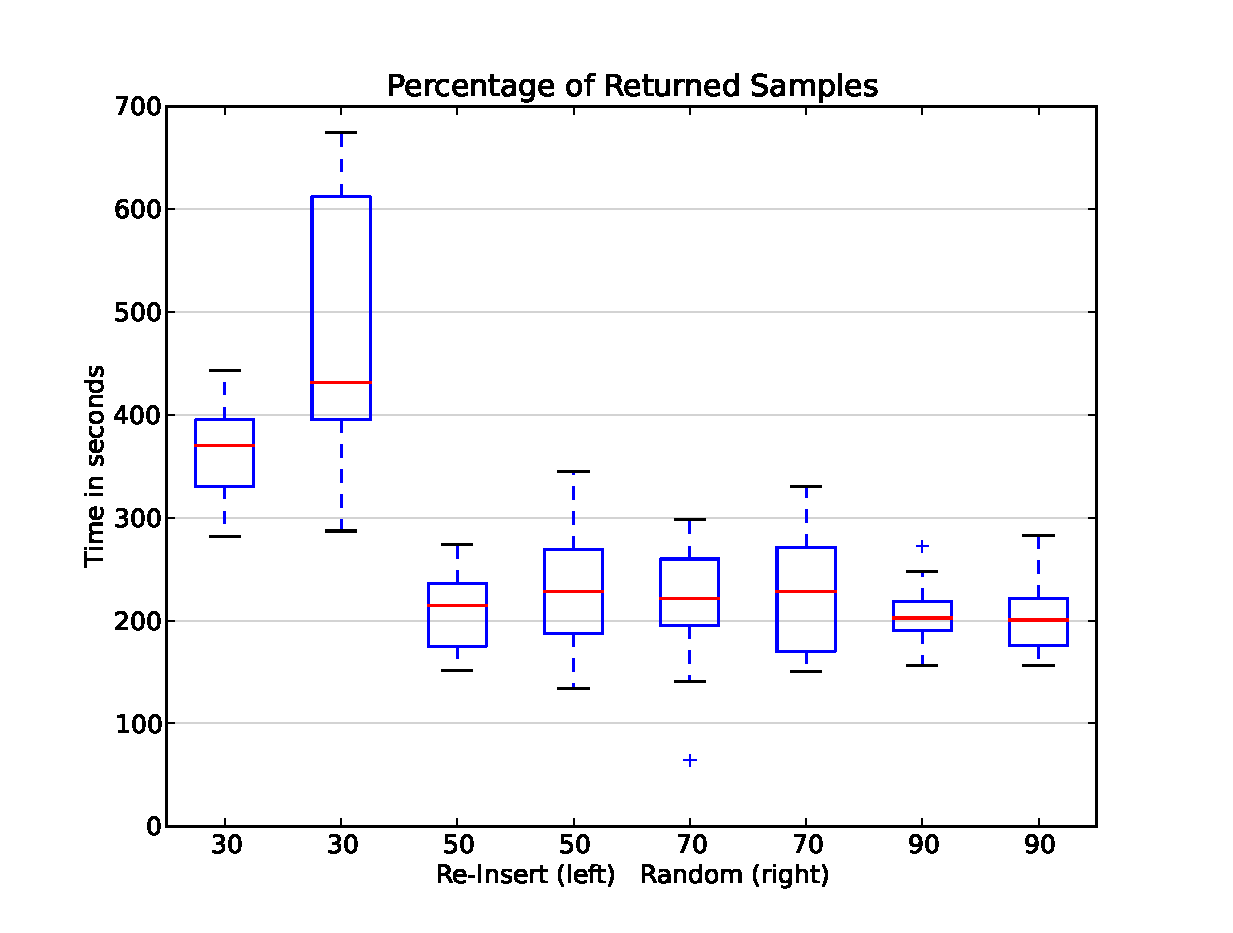
\includegraphics[width=5.9cm]{plot_time_CRS_w16.eps}
        \label{fig:plot_time_ri_w16}
    }
        \subfigure[]
    {
        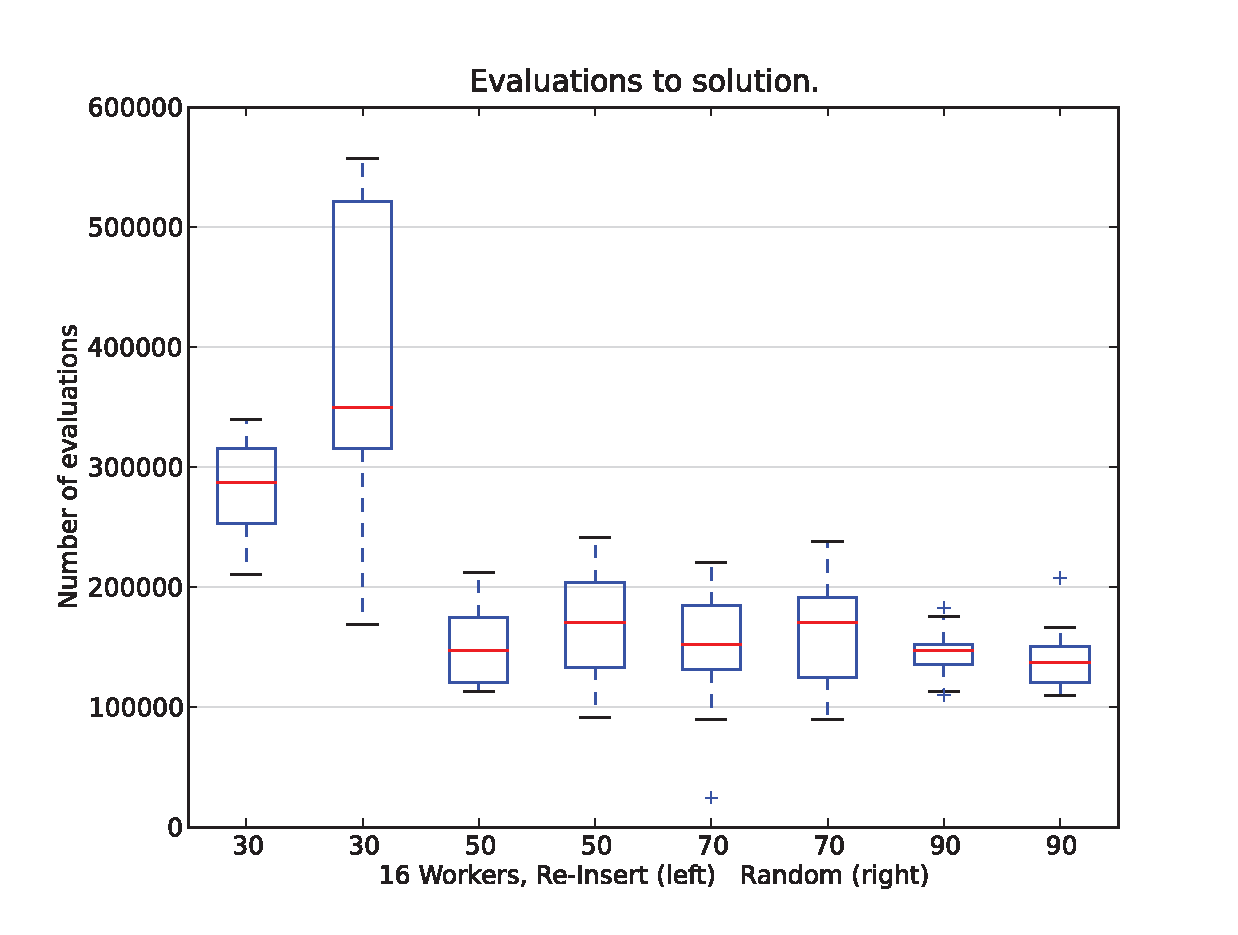
\includegraphics[width=5.9cm]{16_plot_evals.eps}
        \label{fig:plot_evals_w16}
    }
        \subfigure[]
    {
        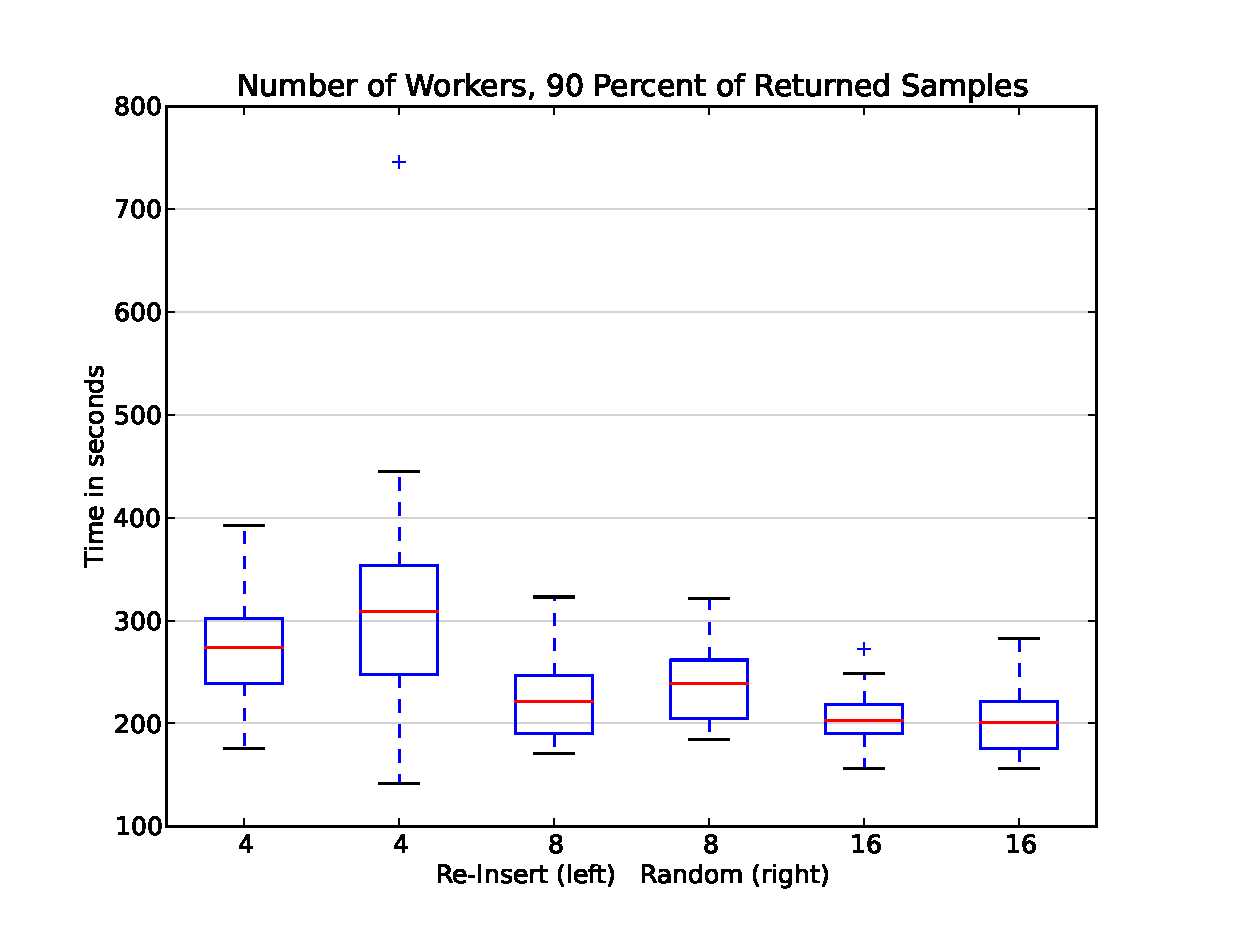
\includegraphics[width=5.9cm]{plot_percent_90.eps}
        \label{fig:plot_percent_90}
    }
        \subfigure[]
    {
        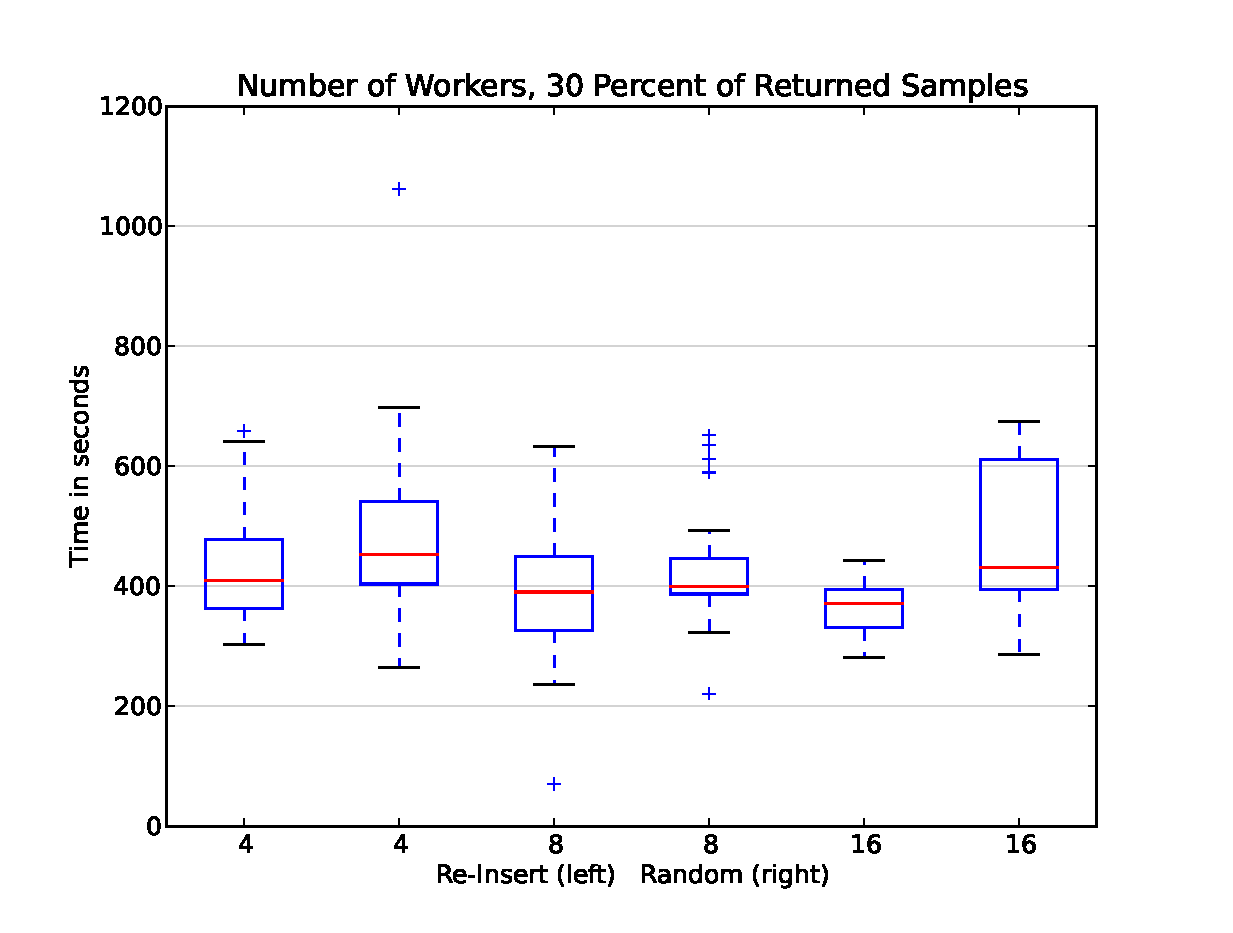
\includegraphics[width=5.9cm]{plot_percent_30.eps}
        \label{fig:plot_percent_30}
    }
    \caption{Unreliable workers: (a) Time to solution, 4 Workers; (b) Time to solution, 8 Worker;
    (c) Time to solution, 16 Workers; (d) Number of evaluations, 16 Workers; (e) Time to solution, 90\% returned samples;
    (f) Time to solution, 30\% returned samples. }
% Please note that max values are higher in the random case, although
% there are more substantial drops. Maximun is also reached
% first. Maybe this should go to the explanation? - JJ 
    \label{fig:effort_unreliable}
\end{figure*}


\begin{figure*}[t]
    \centering
    \subfigure[]
    {
        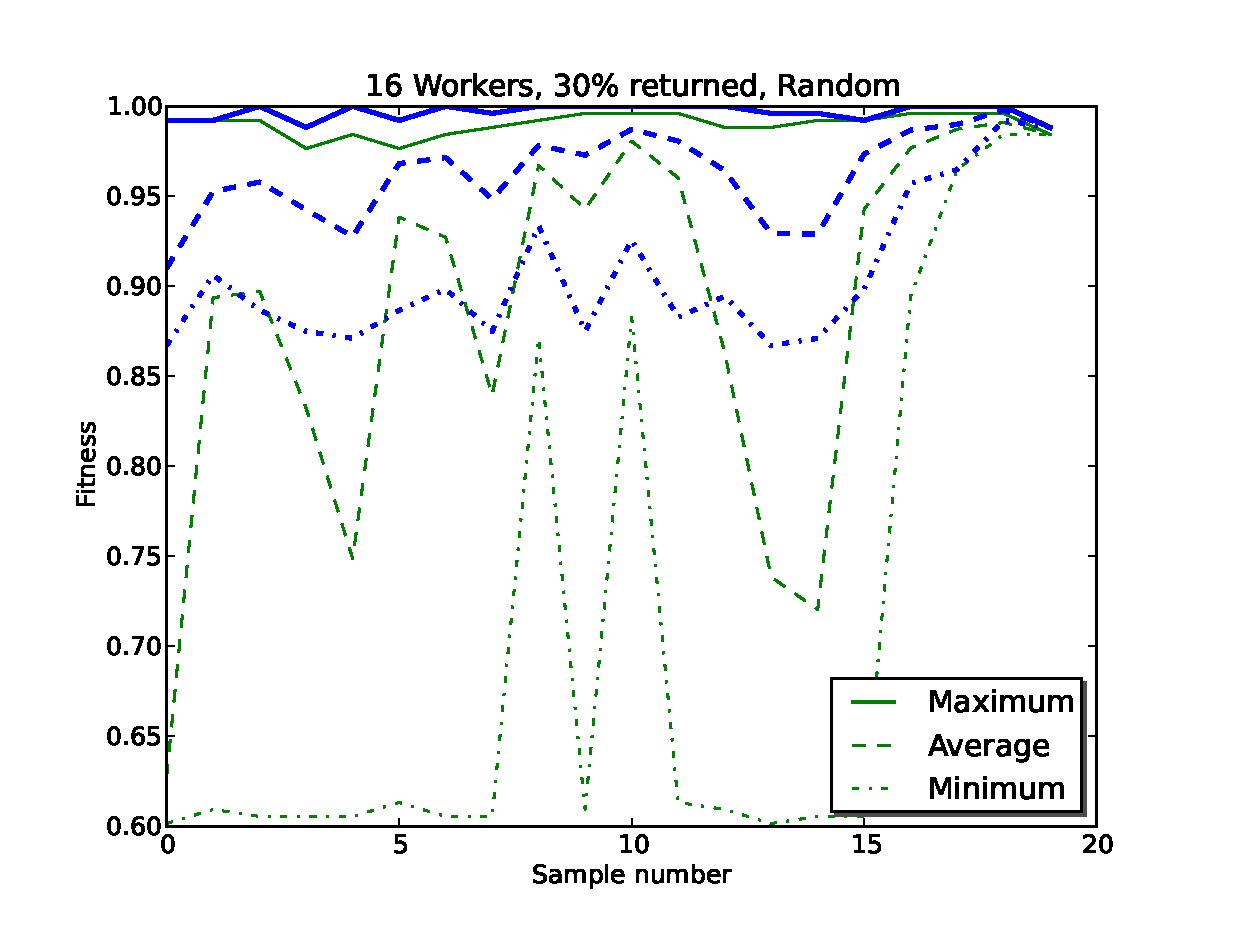
\includegraphics[width=5.9cm]{Fitness-w16-30-random.eps}
        \label{fig:Fitness-w16-30-random}
    }
        \subfigure[]
    {
        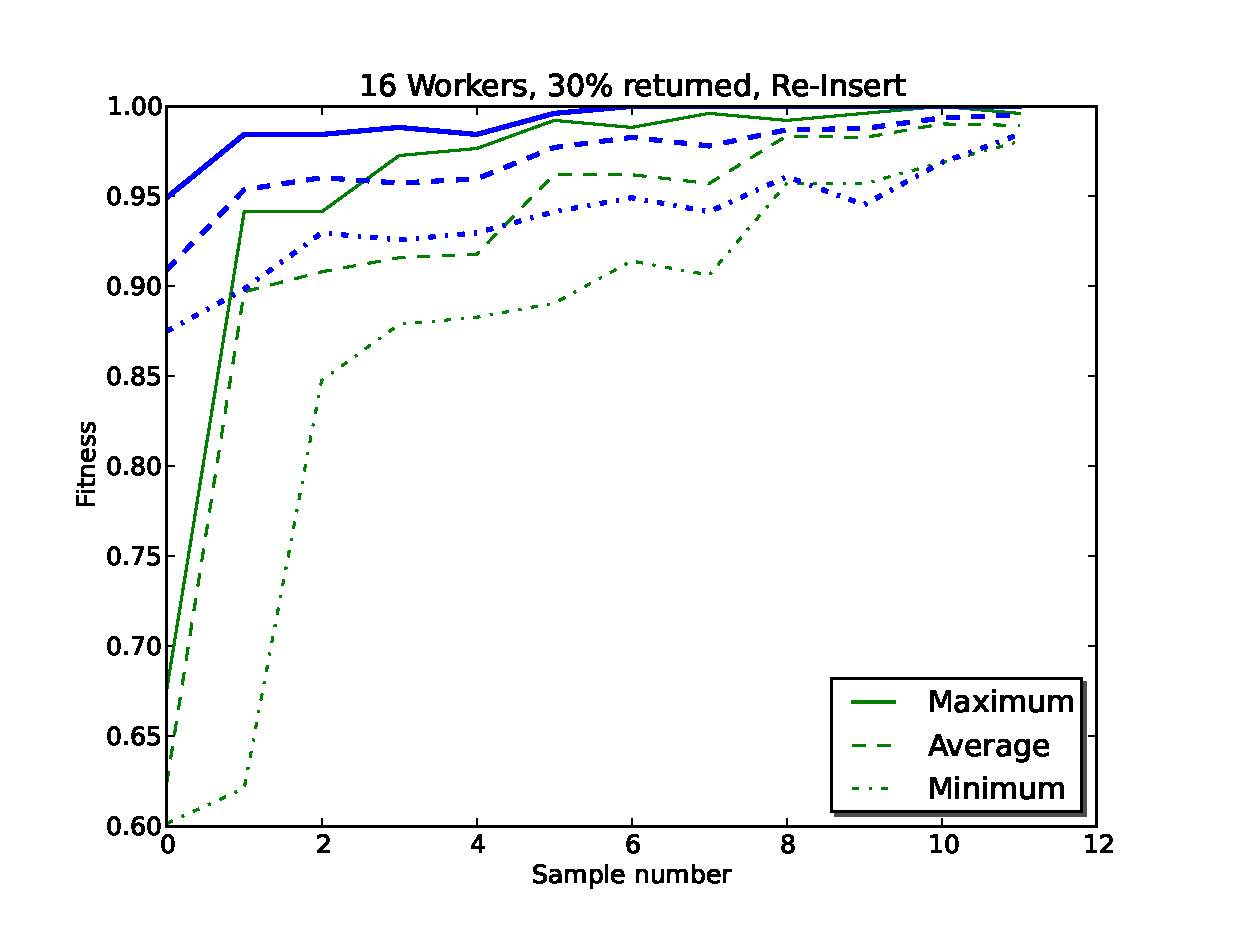
\includegraphics[width=5.9cm]{Fitness-w16-30-reinsert.eps}
        \label{fig:Fitness-w16-30-reinsert}
    }
    \caption{Evolution of fitness with respect to sample number, using 30\% returned samples and 16 Workers,
    for each sample the average fitness was measured at the start (green) and end (blue) of each local evolution, with (a) random algorithm and
    (b) reinsertion algorithm. }
% Please note that max values are higher in the random case, although
% there are more substantial drops. Maximun is also reached
% first. Maybe this should go to the explanation? - JJ 
    \label{fig:effort_unreliable2}
\end{figure*}


Hence, the goal of this section is to evaluate the effect the reinsertion algorithm has on the total
running time and number of evaluations of a GA, using the P-Peaks problem described above with the same parametrization described in Table \ref{tab:paramse};
however, in this case c2 Unreliable Realtime workers are used, which are less efficient than the c1 workers used in Section \ref{expb}.
In particular, two distinct approaches are evaluated: (a) reinserting previously taken individuals, at the cost of keeping copies of
samples; and (b) inserting randomly generated individuals, which has the added effect of increasing diversity within the population.

The algorithm stops when reaching the optimum value, or when all workers
pulled 100 samples. To simulate unreliable workers each worker was assigned a
return sample probability. In the experiments the lower probability was a 30\%
chance of an EvoWorker returning a sample or an EvoWorker failing 70\% of the
time; other return sample probabilities where 50\%, 70\% and 90\%.
Here, it might be said that workers with a low return probability (say 30\%) should in fact be avoided,
and a proper strategy would be to eliminate those workers from the evolutionary process.
However, we consider a scenario were the reliability of a worker is not known a priori, their reliability can only be assessed after an experiment is conducted (or during).
Over time, however, it might be possible to build historic profiles of participating workers at take appropriate steps to improve performance when a highly unreliable
worker is detected, but incorporating such strategies is left as future work.

Experiments where carried out using a total of 4, 8 and 16 EvoWorkers.
Although supported by EvoSpace, time intervals were not chosen as triggers
to feed the population with new individuals, population size was used instead.
The population size is a better threshold as it is more critical
to a GA performance, for instance in experiments where the population remaining in the pool was near starvation, the time to completion increased.
For these experiments, the insertion of individuals was triggered when less than
128 individuals remain in the EvoStore; the number of individuals fed to the
population was 128, or 8 complete samples, when the reinsertion algorithm was used.


Figure~\ref{fig:plot_time_ri_w4} shows the time required 
to solution when using four EvoWorkers. For a population of
512 individuals and a sample size of 16, there is no
difference in the time required to solution for 
percentages of 50\% and above. Both reinsertion algorithms
had comparable times. For 30 percent, both approaches 
had a slight increase in time. For 8 workers, shown in Figure~\ref{fig:plot_time_ri_w8},  there was a marginal
decrease in overall time; and results where similar to those found in the experiments with 4 workers.  
Figure~\ref{fig:plot_time_ri_w16} shows results for 16 workers,
when there was only a 30\% chance of returning a sample the rate of reinsertion was high, this produced one reinsertion event approximately once every 35 samples,
considering that 8 samples were reinserted at every such event.
In this case, the insertion of random individuals resulted in a higher time to solution.

In summary, the results suggest that the reinsertion algorithm is better
for situations when starvation of the pool is common.
On the other hand, inserting random individuals is not detrimental when there
are other evolved individuals within the pool, but when the remaining
pool mainly consists of random individuals, new samples pulled by EvoWorkers need to start the search from scratch. 
Therefore, if only a small number of samples are returned to the pool, the work needed to reach the
optimum is increased. Figure~\ref{fig:plot_evals_w16} also shows the number 
of evaluations needed to reach an optimum for 16 workers.
Figures~\ref{fig:plot_percent_90} and \ref{fig:plot_percent_30} show
the time required to solution for 30\% and 90\% of returned samples, two extreme cases.
For 90\% both algorithms had similar speedups as the number of workers increases.
Conversely, for a return probability of 30\% there is practically no speedup at all with more EvoWorkers.
The reinsert algorithm, however, does show a lower median total time compared with the random strategy, particularly with 4 and 16 EvoWorkers.         

Fitness with respect to time was measured as the average from each consecutive
sample pulled by each worker. For each sample, the average fitness
was measured at the start and at the end of the local evolution.
Also the minimum and maximum fitness values at the start and finish was recorded.    
Figure~\ref{fig:Fitness-w16-30-random} shows the evolution of fitness
with the random insertion algorithm, where the initial fitness drops
at certain points when random insertion occurs, while average final fitness 
is also compromised. Figure~\ref{fig:Fitness-w16-30-reinsert}
shows results for the reinsertion algorithm, with more
characteristic convergence curves without substantial fitness drops. 





\subsection{Parametrization}
In general, EAs are sometimes criticized by the large number of parameters they require,
that need to be tuned empirically or require additional heuristic processes to be included into the search to
adjust the parameters automatically \cite{parameters,ss}.
In the case of a Pool-EAs, this issue is magnified since the underlying system architecture adds several degrees of freedom to the search process,
with unknown interactions.
This problem is of particular importance in real-world scenarios, where there might be little prior insights regarding what could be the best
configuration for an EA tool, especially if the intent is to use it as a black-box optimizer;
a comprehensive survey on this topic is given in \cite{parameters}. 

A noteworthy contribution is made by Cant\'u Paz \cite{cantu}, who addresses the problem of deriving theoretical models of the effects
of parameters related to population size and migration in Island-Model EAs (IMEA).
However, it does not cover the effects of all possible parameters, or the intricacies of a Pool-EA algorithm.
%Here, we would stress some important differences between PEAs and IMEAs.
%First, an IMEA presents a fixed topological structure, with a predefined interaction protocol among each evolving population,
%this leads to a coordinated, or even synchronized, interaction between the islands.
%On the other hand, a Pool-EA does not consider such a structure, the interactions between workers is much less structured or controlled.
%Second, in an IMEA each island represents an individual evolutionary process, sharing some of the same dynamics as standard EAs.
%In a Pool-EA, however, only a single centralized population exists, samples of which are distributed across workers, but ultimately combined once again
%in the centralized pool.
Therefore, some of the well-known insights derived from IMEA research (regarding, for example, migration policies)
are not necessarily relevant in the Pool-EA framework.

Therefore, the recently proposed approach called Randomized Parameter Setting Strategy (RPSS) \cite{fuku1,fuku2}
is tested with EvoSpace in this section.
The idea behind RPSS is that in a distributed EA, algorithm parametrization may be completely skipped to conduct a successful search.
The first works with RPSS focused on an IMEA model \cite{fuku1,fuku2},
where the tuning task can become overwhelming, particularly if the number of islands is large.
Therefore, the proposal in \cite{fuku1} is to set the parameter values randomly, without a tuning or self-adaptive process whatsoever.
The RPSS approach sets the parameters of each deme randomly at the beginning of the run, a very simple and apparently naive approach.
Results suggest that when the number of distributed process is large enough, algorithm parameters can be set randomly and still achieve
good results.
Therefore the goal of this section is to evaluate RPSS on an EvoSpace Pool-EA.

\begin{table}[t]
\renewcommand{\arraystretch}{1.3}
\caption{GA and EvoWorker parameters used in Section 6.2.}
\label{tab:params}
\centering
\begin{tabular}{|l|c|}
\hline
\multicolumn{2}{|c|}{GA Parameters} \\
\hline
Tournament size & 4 \\
Crossover rate & 0.85  \\
Population Size & 512 \\
Mutation probability & 0.5 \\
Independent bit flip probability  & 0.02 \\
\hline
\multicolumn{2}{|c|}{EvoWorker Parameters} \\
\hline
Sample Size & 16 \\
Generations & 128 \\
\hline
\multicolumn{2}{|c|}{Other Parameters} \\
\hline
PiCloud Worker Type & Realtime \\
Number of Workers & 4,8,16 \\
Return Sample Probability & 30\%,50\%,90\% \\
Number of Executions & 30 \\

\hline

\end{tabular}
\end{table}

To gauge the effectiveness of RPSS on a Pool-EA, it is compared with three different parametrization strategies, similar to what is done in \cite{fuku1,fuku2}.
All methods are compared based on average performance over a set of runs.
First, the simplest approach consists on setting all of the EvoWorker parameters homogeneously.
To do this, 200 random parametrizations are created, based on the ranges established in Table \ref{tab:params}.
The average performance of these runs characterizes the random-homogeneous parametrization, denoted Average-Homogeneous.
From these runs, the best configuration is chosen, the one that achieved the best results,
and then 20 independent runs are carried out on each problem, this method is called Best-Homogeneous.
Finally, the random-heterogeneous-parametrization is considered, where the parameters of each worker are set independently at random at
the beginning of each run; 20 independent runs are performed, the method is denoted as Average-Heterogeneous.
The algorithms are evaluated using the P-Peaks problems.

Experiments are carried out using a different number of EvoWorkers on each problem.
The first group of runs are done with $16$ EvoWorkers, and the second with $120$.
Based on \cite{fuku1,fuku2}, it is assumed that with an increased number of workers the RPSS approach will achieve relatively better results, much closer to
the Best-Homogeneous configuration.
This is particularly important, since increasing the number of EvoWorkers greatly magnifies the dimensionality of the tuning problem.
Results are summarized by tracking how the best solution found so far varies with respect to the total
number of samples taken from the EvoStore.
These results are presented in Figure \ref{fig:PPeaks}, showing the average performance for each of the three methods.

\begin{figure}[t]
    \centering
    	\subfigure[16 EvoWorkers]
    {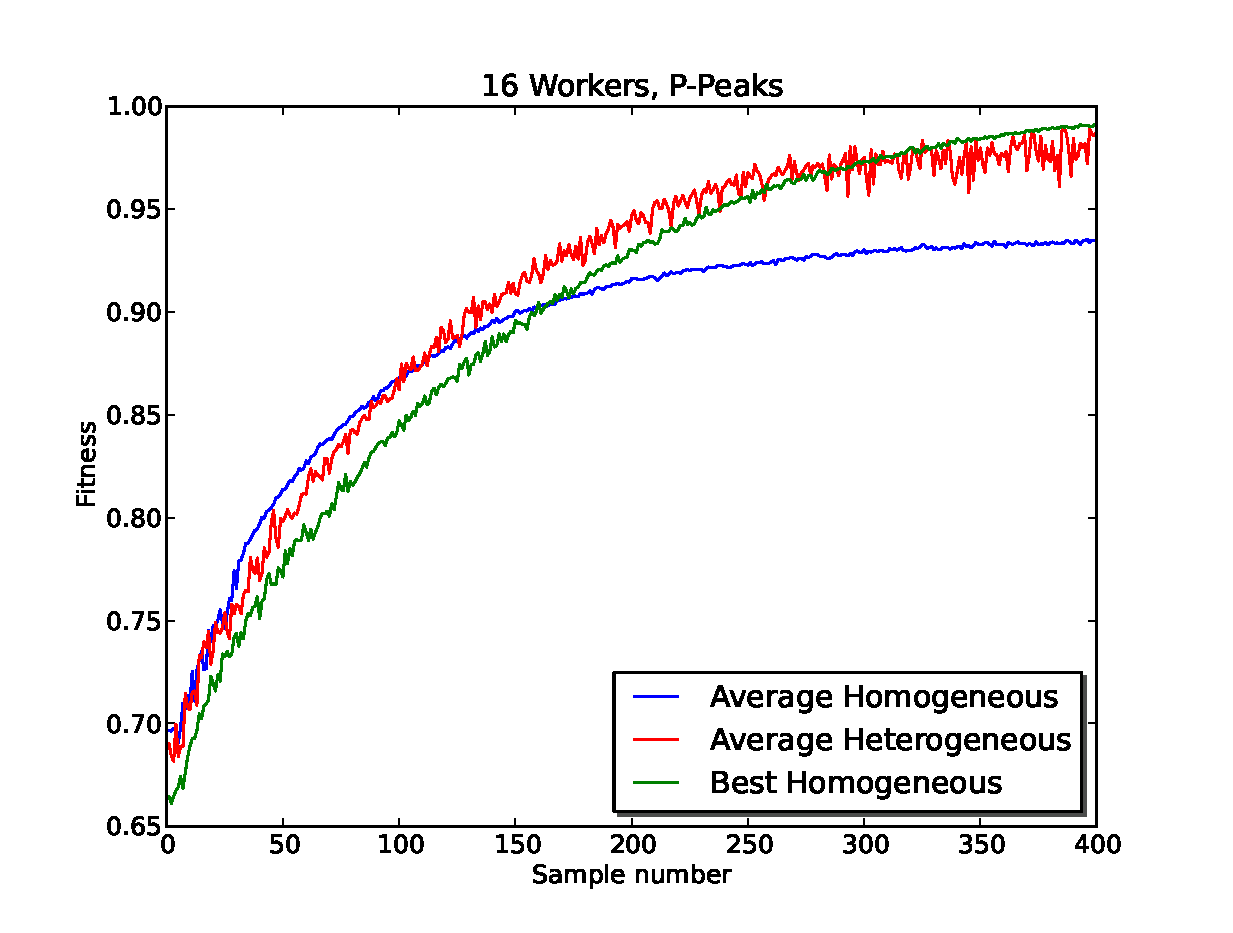
\includegraphics[width=5.9cm]{PPeaks-w16.eps}}
        \subfigure[120 EvoWorkers]
    {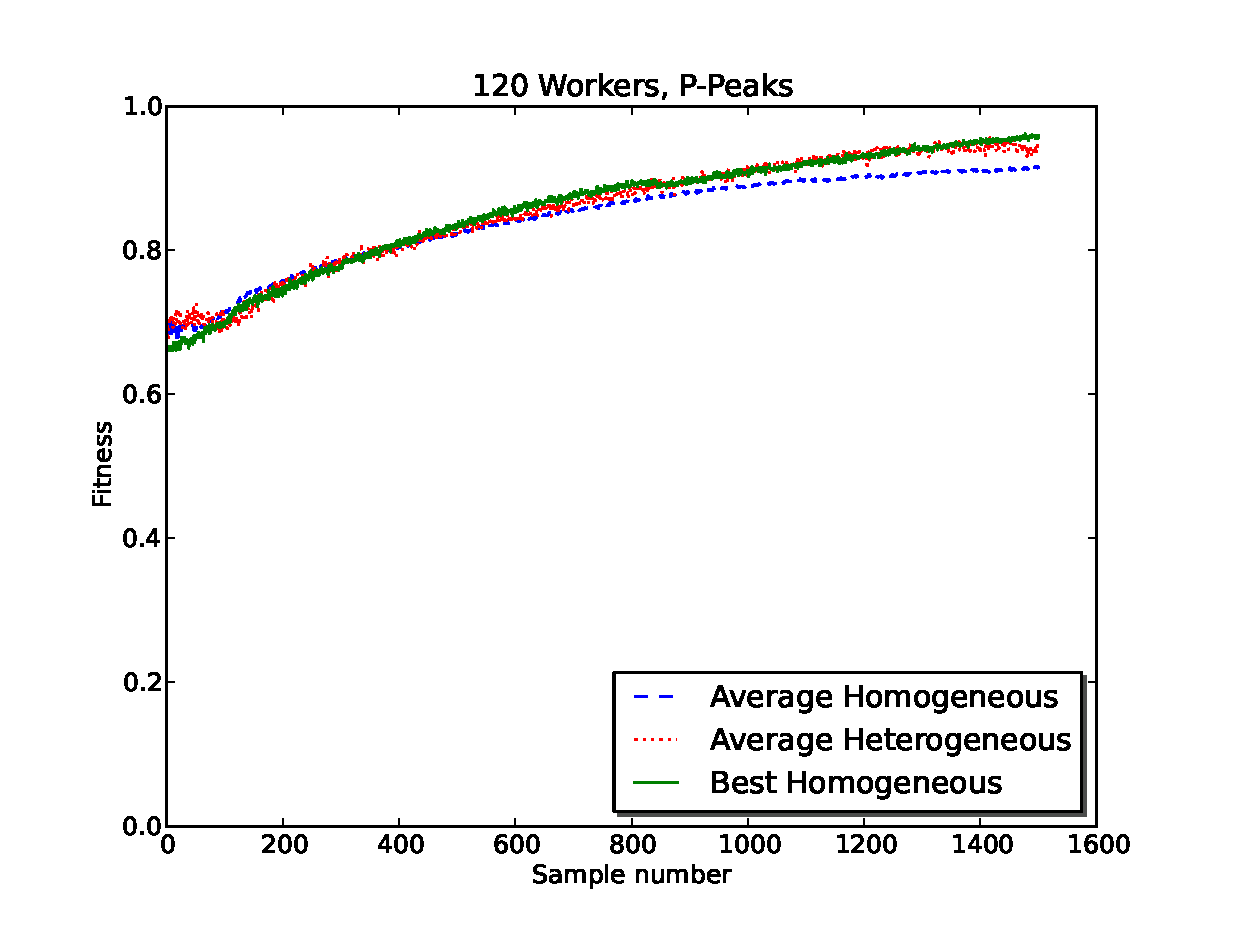
\includegraphics[width=5.9cm]{PPeaks-w120.eps}}
    \caption{Convergence plots for the P-Peaks with 16 (a) and 120 (b)
      EvoWorkers .}
% Both plots should use the same x-axis; it''s misleading otherwise -
% JJ 
    \label{fig:PPeaks}
\end{figure}



First, with 16 EvoWorkers we can see a clear trend, the Average Heterogeneous configuration is similar with the Best Homogeneous configuration,
depicted in Figure \ref{fig:PPeaks}(a).
This is a promising result, since the heterogeneous configuration did not require any parameter tuning, while the best homogeneous configuration
is chosen from a set of 200 runs.
Moreover, the plots show that using an homogeneous configuration with random values achieves noticeably inferior performance.
When the number of EvoWorkers is increased, which is shown in Figure \ref{fig:PPeaks}(b), a similar trend appears,
however the differences among the algorithms is reduced.
Future work will compare this technique with other known parametrization methods \cite{cantu}, to determine the best
parametrization strategies for a wider range of EAs and problem domains. 
Nevertheless, these results suggest that a random heterogeneous parametrization following the RPSS approach could be used as a simple off-the-shelf
parametrization approach for practitioners interested in using the ESM.

%\subsection{Discussion}


\section{Concluding Remarks}
\label{sec:conclusions}
This paper presents the EvoSpace model for the development of pool-based EAs, which is designed to exploit computing resources over a network and can be implemented to run directly on the cloud.
Pool-EAs present several interesting properties that are not present in standard EAs, storing the population in a central store and
performing the evolutionary process in an asynchronous and distributed manner through client machines,
which in the ESM are referred to as EvoWorkers.
In this sense, what is particularly interesting of a Pool-EA is that it incorporates features from natural evolution that are abstracted away in common EA implementations.
Moreover, they are intended as means by which evolutionary computation techniques can incorporate modern computing frameworks.
However, Pool-EAs also present several noteworthy design challenges, that must be addressed.
The proposed ESM is intended as a conceptual framework that addresses some of these challenges and allows for the development of a variety of search techniques
that follow this pool-based approach.

At the implementation level, this work also presents an ESM instantiation called EvoSpace-py, a software tool that simplifies the deployment of Pool-EAs,
as multi-threaded processes or on the cloud.
The system has been programmed using the Python programming language, the DEAP library and the Redis key-value database.

Experimental results are presented for a pool-based GA, using standard benchmarks and comparing the system with a standard GA search and an IMEA.
Results are encouraging in several respects.
First, it seems that the ESM can perform a more efficient search that an IMEA, requiring about half as many fitness function evaluations to find
a solution on a standard benchmark.
Second, performance of the ESM is equivalent or better than standard search, with the added benefit of improved efficiency
and population diversity.
Third, results illustrate the benefits of adding client workers to the evolutionary process.
Fourth, several apparent issues with the Pool-EA approach are studied, regarding the lost connection of unreliable workers and the increased size of the algorithm's parameter space.
In both cases, experimental results suggest that the ESM can handle both issues robustly, using built-in mechanisms and a simple
parametrization strategy.

This paper is the first to comprehensively describe and contextualize the ESM and provides a comprehensive evaluation with respect to standard evolutionary search.
Future work will have to explore the limits and comparative benefits of the ESM,
in order to define the proper domain of competence of Pool-EAs in general and the ESM in particular.
Moreover, the ESM will be leveraged to implement and deploy a complete web-based Pool-EA, that simplifies the use for other researchers in an easy to setup manner.


\section*{Acknowledgements}
Funding provided by CONACYT (Mexico) Project No. 29537 from the Programa de Estimulo a la Innovaci\'on, CONACYT
Basic Science Research Project No. 178323, DGEST (Mexico) Research Projects No.5149.13-P and TIJ-ING-2012-110,
and IRSES project ACoBSEC from the European Commission.
Additional funding provided by projects P08-TIC-03903 (Andalusian Regional Government), TIN2011-28627-C04-02 (Spanish Ministry of Science and Innovation),
project 83 (CANUBE) awarded by the CEI-BioTIC UGR. Regional Government Junta de Extremadura, Consejer\'ia de Econom\'ia, Comercio e Innovaci\'on and FEDER, project GRU10029.


%\begin{acknowledgements}
%If you'd like to thank anyone, place your comments here
%and remove the percent signs.
%\end{acknowledgements}

% BibTeX users please use one of
%\bibliographystyle{spbasic}      % basic style, author-year citations
%\bibliographystyle{spphys} 



%\bibliographystyle{spmpsci}      % mathematics and physical sciences
%\bibliographystyle{spphys}       % APS-like style for physics
%\bibliography{biblio}   % name your BibTeX data base
%
%
\begin{thebibliography}{10}
\providecommand{\url}[1]{{#1}}
\providecommand{\urlprefix}{URL }
\expandafter\ifx\csname urlstyle\endcsname\relax
  \providecommand{\doi}[1]{DOI \discretionary{}{}{}#1}\else
  \providecommand{\doi}{DOI \discretionary{}{}{}\begingroup
  \urlstyle{rm}\Url}\fi

\bibitem{Foster:1998}
I.~Foster, C.~Kesselman (eds.), \emph{The Grid: Blueprint for a New Computing
  Infrastructure} (Morgan Kaufmann Publishers Inc., San Francisco, CA, USA,
  1999)

\bibitem{Baxevanidis:2002}
K.~Baxevanidis, H.~Davies, I.~Foster, F.~Gagliardi, Comput. Netw.
  \textbf{40}(1), 5 (2002)

\bibitem{cloud}
M.~Armbrust, A.~Fox, R.~Griffith, A.D. Joseph, R.~Katz, A.~Konwinski, G.~Lee,
  D.~Patterson, A.~Rabkin, I.~Stoica, M.~Zaharia, Commun. ACM \textbf{53}(4),
  50 (2010)

\bibitem{varia2008cloud}
J.~Varia, White Paper of Amazon  (2008)

\bibitem{Oram:2001}
A.~Oram (ed.), \emph{Peer-to-Peer: Harnessing the Power of Disruptive
  Technologies} (O'Reilly \& Associates, Inc., Sebastopol, CA, USA, 2001)

\bibitem{Curbera:2002}
F.~Curbera, M.~Duftler, R.~Khalaf, W.~Nagy, N.~Mukhi, S.~Weerawarana, IEEE
  Internet Computing \textbf{6}(2), 86 (2002)

\bibitem{sofea1}
J.J. Merelo-Guerv\'{o}s, A.~Mora, J.A. Cruz, A.I. Esparcia, in
  \emph{Proceedings of the 2012t European conference on Applications of
  Evolutionary Computation} (Springer-Verlag, Berlin, Heidelberg, 2012),
  EvoApplications'12, pp. 446--455

\bibitem{sofea2}
J.J. Merelo-Guervos, A.~Mora, J.A. Cruz, A.I. Esparcia-Alcazar, C.~Cotta, in
  \emph{2012 IEEE Congress on Evolutionary Computation (CEC)} (IEEE Comuter
  Society, 2012), pp. 1 --8

\bibitem{sofea3}
J.J. Merelo, C.M. Fernandes, A.M. Mora, A.I. Esparcia, in \emph{Proceedings of
  the 14th Annual Conference Companion on Genetic and Evolutionary Computation}
  (ACM, New York, NY, USA, 2012), GECCO '12, pp. 109--116

\bibitem{PoolvsIsland}
J.J. Merelo, A.~Mora, C.~Fernandes, A.~Esparcia-Alcazar, J.~Laredo, in
  \emph{P2P, Parallel, Grid, Cloud and Internet Computing (3PGCIC), 2012
  Seventh International Conference on} (2012), pp. 19--24

\bibitem{Evospace}
M.~Garc{\'\i}a-Valdez, L.~Trujillo, F.~Fern{\'a}ndez~de Vega, J.J.
  Merelo~Guerv\'os, G.~Olague, in \emph{Applications of Evolutionary
  Computation}, \emph{LNCS}, vol. 7835, ed. by A.~Esparcia-Alc{\'a}zar, et~al.
  (Springer Berlin Heidelberg, 2013), pp. 499--508

\bibitem{Musart}
M.~Garcia-Valdez, L.~Trujillo, F.~Fern{\'a}ndez~de Vega, J.~Merelo~Guerv{\'o}s,
  G.~Olague, in \emph{Evolutionary and Biologically Inspired Music, Sound, Art
  and Design}, \emph{LNCS}, vol. 7834, ed. by P.~Machado, et~al. (Springer
  Berlin Heidelberg, 2013), pp. 121--130

\bibitem{FreeLunch}
M.~Garcia-Valdez, A.~Mancilla, L.~Trujillo, J.J. Merelo, F.~Fernandez-de Vega,
  in \emph{2013 IEEE Congress on Evolutionary Computation (CEC)} (2013), pp.
  1255--1262

\bibitem{Fire}
L.~Trujillo, M.G. Valdez, F.F. de~Vega, J.J. Merelo-Guerv\'os, in \emph{IEEE
  Congress on Evolutionary Computation} (IEEE, 2013), pp. 2871--2878

\bibitem{linda}
D.~Gelernter, ACM Trans. Program. Lang. Syst. \textbf{7}(1), 80 (1985)

\bibitem{eiben}
A.E. Eiben, J.E. Smith, \emph{Introduction to Evolutionary Computing}
  (SpringerVerlag, 2003)

\bibitem{parallelEA}
E.~Alba, \emph{Parallel Metaheuristics: {A} New Class of Algorithms} (John
  Wiley \& Sons, 2005)

\bibitem{spector:2007}
J.~Klein, L.~Spector, in \emph{Proceedings of the 9th annual conference on
  Genetic and evolutionary computation} (ACM, New York, NY, USA, 2007), GECCO
  '07, pp. 1628--1635

\bibitem{merelo:2008}
J.J. Merelo~Guervos, P.A.C. Valdivieso, J.L.J. Laredo, A.M. Garc{\'\i}a,
  A.~Prieto, in \emph{IEEE Congress on Evolutionary Computation} (IEEE, 2008),
  pp. 1372--1379

\bibitem{cotillon:2012}
A.~Cotillon, P.~Valencia, R.~Jurdak, in \emph{Proceedings of the 15th European
  conference on Genetic Programming} (Springer-Verlag, Berlin, Heidelberg,
  2012), EuroGP'12, pp. 13--24

\bibitem{langdon:2004}
W.B. Langdon, in \emph{Genetic Programming, Proceedings of EuroGP'2004},
  \emph{LNCS}, vol. 3003, ed. by M.~Keijzer, U.M. O'Reilly, S.M. Lucas,
  E.~Costa, T.~Soule (Springer-Verlag, 2004), \emph{LNCS}, vol. 3003, pp.
  349--358

\bibitem{picbreeder}
J.~Secretan, N.~Beato, D.B. D'Ambrosio, A.~Rodriguez, A.~Campbell, J.T.
  Folsom-Kovarik, K.O. Stanley, Evol. Comput. \textbf{19}(3), 373 (2011)

\bibitem{MilkyWay}
N.~Cole, T.J. Desell, D.L. Gonzalez, F.F. de~Vega, M.~Magdon-Ismail, H.J.
  Newberg, B.K. Szymanski, C.A. Varela, in \emph{Parallel and Distributed
  Computational Intelligence}, \emph{Studies in Computational Intelligence},
  vol. 269 (Springer, 2010), pp. 63--90

\bibitem{nc}
F.~Fern\'{a}ndez De~Vega, G.~Olague, L.~Trujillo, D.~Lombra\~{n}a Gonz\'{a}lez,
  Natural Computing \textbf{12}(2), 163 (2013)

\bibitem{garcia2011}
M.~Garcia-Arenas, J.J. Merelo, A.M. Mora, P.~Castillo, G.~Romero, J.~Laredo, in
  \emph{2011 IEEE Congress on Evolutionary Computation (CEC)} (IEEE, 2011), pp.
  304--311

\bibitem{DREAM}
B.~Paechter, T.~Back, M.~Schoenauer, M.~Sebag, A.~Eiben, J.J. Merelo,
  T.~Fogarty, in \emph{Evolutionary Computation, 2000. Proceedings of the 2000
  Congress on}, vol.~2 (2000), vol.~2, pp. 951--958 vol.2

\bibitem{ParadisEO}
S.~Cahon, N.~Melab, E.G. Talbi, Journal of Heuristics \textbf{10}(3), 357
  (2004)

\bibitem{free-form}
M.~Schmidt, H.~Lipson, Science \textbf{324}, 81 (2009)

\bibitem{VecchiolaCORR}
C.~Vecchiola, M.~Kirley, R.~Buyya, CoRR \textbf{abs/0903.1386} (2009)

\bibitem{FlexGP}
D.~Sherry, K.~Veeramachaneni, J.~McDermott, U.M. O'Reilly, in
  \emph{Applications of Evolutionary Computation}, \emph{LNCS}, vol. 7248, ed.
  by C.~di~Chio, et~al. (Springer Berlin Heidelberg, 2012), pp. 477--486

\bibitem{cantu}
E.~Cant\'u-Paz, in \emph{Parameter Setting in Evolutionary Algorithms},
  \emph{Studies in Computational Intelligence}, vol.~54, ed. by F.G. Lobo, C.F.
  Lima, Z.~Michalewicz (Springer, 2007), pp. 259--276

\bibitem{ateam}
S.~Talukdar, L.~Baerentzen, A.~Gove, P.~De~Souza, Journal of Heuristics
  \textbf{4}(4), 295 (1998)

\bibitem{roy:2009}
G.~Roy, H.~Lee, J.L. Welch, Y.~Zhao, V.~Pandey, D.~Thurston, in
  \emph{Proceedings of the Eleventh conference on Congress on Evolutionary
  Computation} (IEEE Press, Piscataway, NJ, USA, 2009), CEC'09, pp. 1177--1184

\bibitem{bollini:1999}
A.~Bollini, M.~Piastra, in \emph{Proceedings of the Second European Workshop on
  Genetic Programming} (Springer-Verlag, London, UK, UK, 1999), pp. 173--183

\bibitem{DEAP_JMLR2012}
F.A. Fortin, F.M.D. Rainville, M.A. Gardner, M.~Parizeau, C.~Gagn\'e, Journal
  of Machine Learning Research \textbf{13}, 2171 (2012)

\bibitem{trap}
D.~Thierens, Evolutionary Computation \textbf{7}, 331 (1999)

\bibitem{Jong:PS97}
K.A. De~Jong, M.A. Potter, W.M. Spears, in \emph{ICGA}, ed. by T.~B\"ack
  (Morgan Kaufmann, 1997), pp. 338--345

\bibitem{nodeo}
J.J. Merelo, P.~Castillo, A.~Mora, A.~Esparcia-Alc{\'a}zar, V.~Rivas-Santos, in
  \emph{Proceedings of the 2014 conference companion on Genetic and
  evolutionary computation companion} (ACM, 2014), pp. 1155--1162

\bibitem{diversity}
R.W. Morrison, K.A.D. Jong, in \emph{Selected Papers from the 5th European
  Conference on Artificial Evolution} (Springer-Verlag, London, UK, UK, 2002),
  pp. 31--41

\bibitem{Jong:1990}
K.A. De~Jong, W.M. Spears, in \emph{Proceedings of the 1st Workshop on Parallel
  Problem Solving from Nature} (Springer-Verlag, London, UK, UK, 1991), PPSN I,
  pp. 38--47.

\bibitem{sofea:naco}
J.J. Merelo, A.~Mora, C.~Fernandes, A.I. Esparcia-Alc{\'a}zar, Natural
  Computing pp. 1--14 (2012)

\bibitem{fazenda2012}
P.~Fazenda, J.~McDermott, U.M. O'Reilly, in \emph{Applications of Evolutionary
  Computation}, \emph{LNCS}, vol. 7248, ed. by C.~di~Chio, et~al. (Springer
  Berlin Heidelberg, 2012), \emph{LNCS}, vol. 7248, pp. 416--425

\bibitem{parameters}
F.G. Lobo, C.F. Lima, Z.~Michalewicz, \emph{Parameter Setting in Evolutionary
  Algorithms} (Springer Publishing Company, Incorporated, 2007)

\bibitem{ss}
O.~Kramer, \emph{Self-Adaptive Heuristics for Evolutionary Computation},
  \emph{Studies in Computational Intelligence}, vol. 147 (Springer, 2008)

\bibitem{fuku1}
Y.~Gong, A.~Fukunaga, in \emph{IEEE Congress on Evolutionary Computation}
  (IEEE, 2011), pp. 820--827

\bibitem{fuku2}
R.~Tanabe, A.~Fukunaga, in \emph{IEEE Congress on Evolutionary Computation}
  (IEEE, 2013), pp. 1263--1270

\end{thebibliography}





\end{document}
% end of file template.tex

